\subsection{Jianqing's summary}
\subsubsection{Fast autoaugment details}
Let $\mathbb{O}$ be a set of augmentation (image transformation) operations
$\mathcal{O}$:$\mathcal{X}\rightarrow\mathcal{X}$ defined on the input image space $\mathcal{X}$. Each operation $\mathcal{O}$ have two parameters: the calling probability $p$ and the magnitude $\lambda$ which determines the variability of operation. Let $\mathcal{S}$ be the set of sub-policies where a sub-policy $\tau \in \mathcal{S}$ consists of $N_{\tau}$ consecutive operations
\{$\mathcal{O}_n^{(\tau)}$($x$;$p_n^{(\tau)}$,$\lambda_n^{(\tau)}$):$n$=1,\ldots,$N_\tau$\}
$$\mathcal{O}(x;p,\lambda):=\left\{
\begin{aligned}
\mathcal{O}(x;\lambda) &&with&&probability&& p \\
x&&with&&probability&&1-p
\end{aligned}
\right.
$$
The output of sub-policy $\tau(x)$ can be described by a composition of operations as:\\
\begin{equation}
\tilde{x}_{(n)}=\mathcal{O}_n^{(\tau)}(\tilde{x}_{(n-1)}),n=1,\ldots,N_{\tau}
\end{equation}

Figure 1 shows a specific example of augmented images by $\tau$ .
Note that each sub-policy $\tau$ is a random sequence of image transformations which depend on $p$ and $\lambda$,and this enables to cover a wide range of data augmentations.
\begin{figure}[H]
	\centering
	% Requires \usepackage{graphicx}
	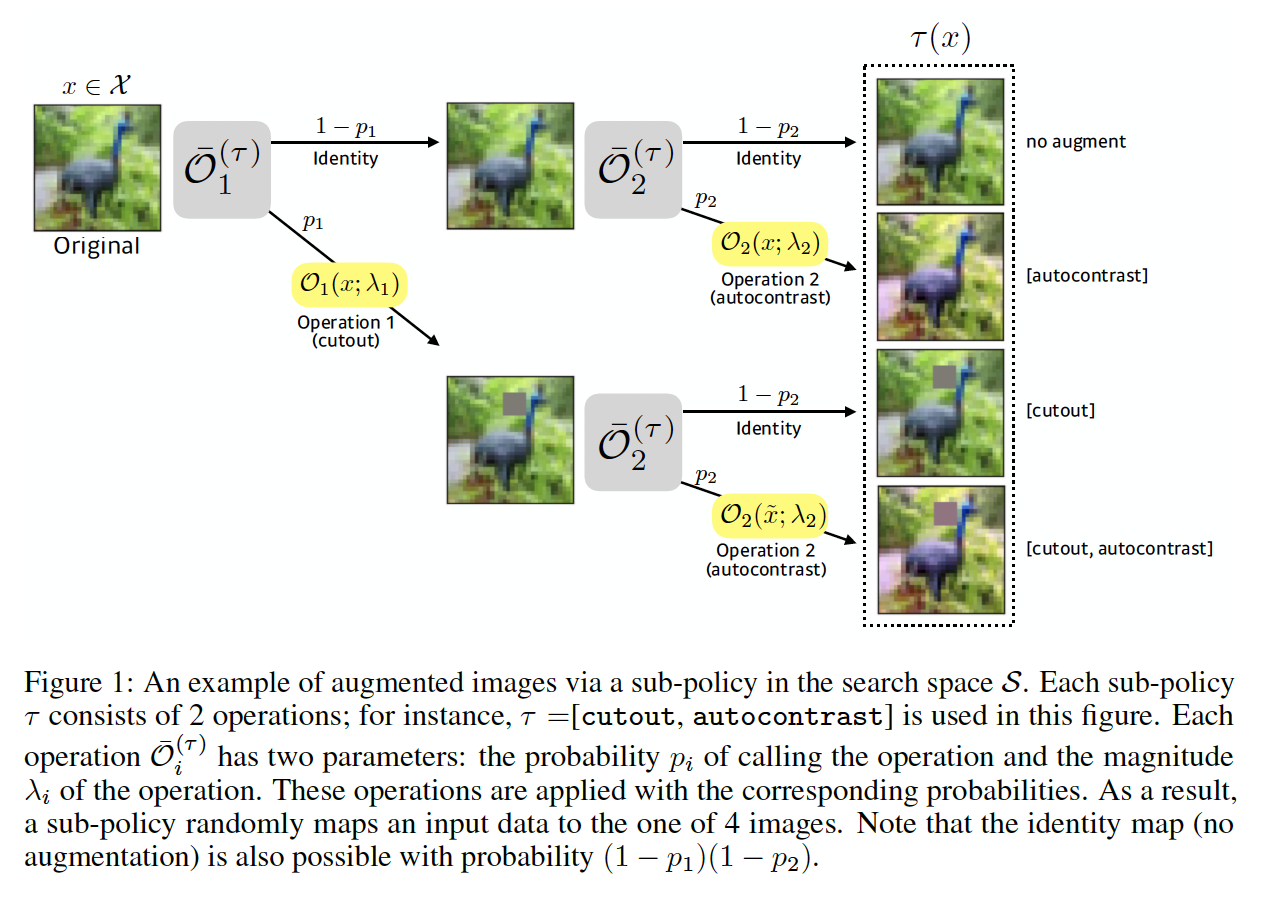
\includegraphics[width=14cm]{fast_fig_1.jpg}
	%  %\caption{}\label{}
\end{figure}

Final policy $T$ is a collection of $N_T$ sub-policies and $T(D)$ indicates a set of augmented images of dataset $D$ transformed by every
sub-policies $\tau\in T$ :
\begin{equation}
T(D)=\cup_{\tau \in T}\{(\tau(x),y):(x,y)\in D\}
\end{equation}
Use both continuous values of probability $p$ and magnitude $\lambda$ at $[0; 1]$ which has more possibilities than discretized search space.


Consider searching the augmentation policy as a density matching between
a pair of datasets. Let $\mathcal{D}$ be a probability distribution on $\mathcal{X}\times\mathcal{Y}$ and assume dataset $D$ is sampled
from this distribution. For a given classification model $\mathcal{M}(\cdot|\theta)$ : $\mathcal{X}\times\mathcal{Y}$ that is parameterized by $\theta$, the expected accuracy and the expected loss of $\mathcal{M}(\cdot|\theta)$ on dataset $D$ are denoted by $\mathcal{R}(\theta |D)$ and $\mathcal{L}(\theta |D)$.

For any given pair of $D_{train}$ and $D_{valid}$, our goal is to improve the generalization ability by searching
the augmentation policies that match the density of $D_{train}$ with density of augmented $D_{valid}$.
It is impractical to compare these two distributions directly for an evaluation of every candidate policy.
Perform this evaluation by measuring how much one dataset follows the pattern of the other by making use of the model predictions on both datasets.

Split $D_{train}$ into $D_{M}$ and $D_{A}$ that are used for learning the model parameter $\theta$ and exploring the augmentation policy $T$.Employ the following objective to find a set of learned augmentation policies
\begin{equation}
T_{*}=argmax_T \mathcal{R}(\theta^*|T(D_A))
\end{equation}
where model parameter $\theta^*$ is trained on $D_{M}$.It is noted that in this objective, $T_{*}$ approximately minimizes the distance between density of $D_{M}$ and density of $T(D_A)$ from the perspective of maxmizing the performance of both model predictions with the same parameter $\theta$.
\begin{figure}[H]
	\centering
	% Requires \usepackage{graphicx}
	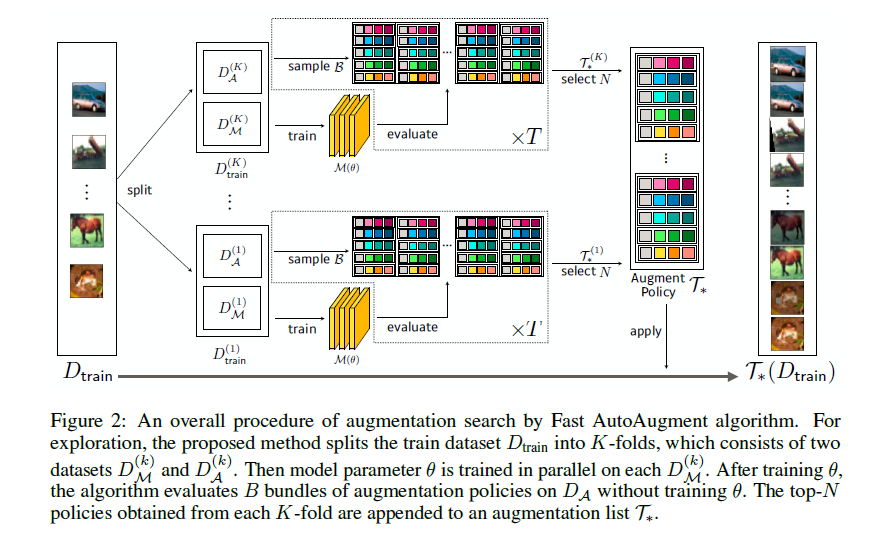
\includegraphics[width=14cm]{fast_fig_2.jpg}
	%  %\caption{}\label{}
\end{figure}

To achieve (3), we propose an efficient strategy for augmentation policy search (see Figure 2). First,we conduct the K-fold stratified shuffling to split the train dataset into $D_{train}^{(1)},...,D_{train}^{(m)}$ where each $D_{train}^{(k)}$ consists of two datasets $D_M^{k}$ and $D_A^{k}$. Next, we train model parameter $\theta$ on $D_M$ from scratch without data augmentation.

After training the model parameter,for each step $1\leq t\leq T$, explore $B$ candidate policies
$\mathcal{B}=\{T_1,\ldots,T_B\}$via Bayesian optimization method which repeatedly samples a sequence of
sub-policies from search space $\mathcal{S}$ to construct a policy $T=\{\tau_1,\ldots,\tau_{N_\tau}\}$ and tunes corresponding
calling probabilities $\{p_1,\ldots,p_{N_\tau}\}$ and magnitudes $\{\lambda_1,\ldots,\lambda_{N_\tau}\}$ to minimize the expected loss
$\mathcal{L}(\theta |\cdot)$ on augmented dataset $T(D_A)$.

As the algorithm completes the exploration step, select top-N policies over $\mathcal{B}$ and denote them $T_t$,Finally, merge every $T_t$ into $T_*$. Augment the whole dataset $D_{train}$ with $T_*$ and retrain the model parameter $\theta$.Through the proposed method, we can expect the performance $\mathcal{R}(\theta|\cdot)$ on augmented dataset $T_*(D_A)$
is statistically higher than that on $D_A$:
\begin{equation}
\mathcal{R}(\theta|T_*(D_A))\geq\mathcal{R}(\theta|D_A)
\end{equation}

\begin{figure}[H]
	\centering
	% Requires \usepackage{graphicx}
	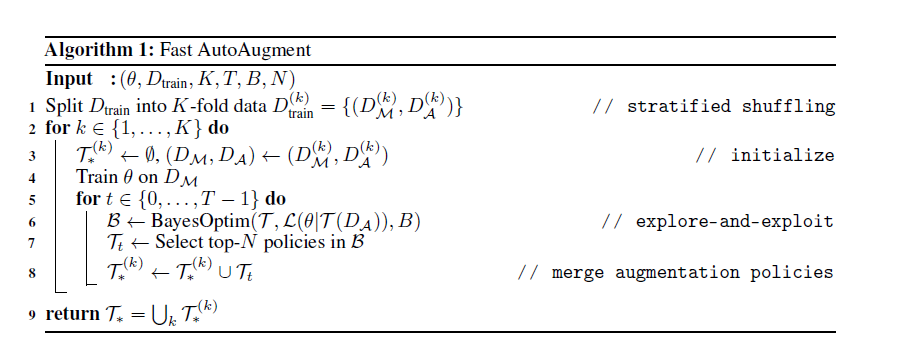
\includegraphics[width=14cm]{fast_fig_3.jpg}
	%  %\caption{}\label{}
\end{figure}

\subsubsection{SGDR}
\begin{equation}
\eta_t = \eta_{min} + \frac{1}{2}(\eta_{max} - \eta_{min})\left(1 +\cos\left(\frac{T_{cur}}{T_{i}}\pi\right)\right)
\end{equation}

where $\eta_{min}^i$ and $\eta_{max}^i$  are ranges for the learning rate, and $T_{cur}$ accounts for how many epochs have been performed since the last restart. Since $T_{cur}$ is updated at each batch iteration $t$. Thus, $\eta_t = \eta_{max}^i$ when $t = 0$ and $T_{cur} = 0$. Once $T_{cur} = T_i$, the cos function will output $-1$ and thus $\eta_t = \eta_{min}^i$. The decrease of the learning rate is shown in Figure 4 for fixed $T_i = 50$, $T_i = 100$ and $T_i = 200$.
\begin{figure}[H]
	\centering
	% Requires \usepackage{graphicx}
	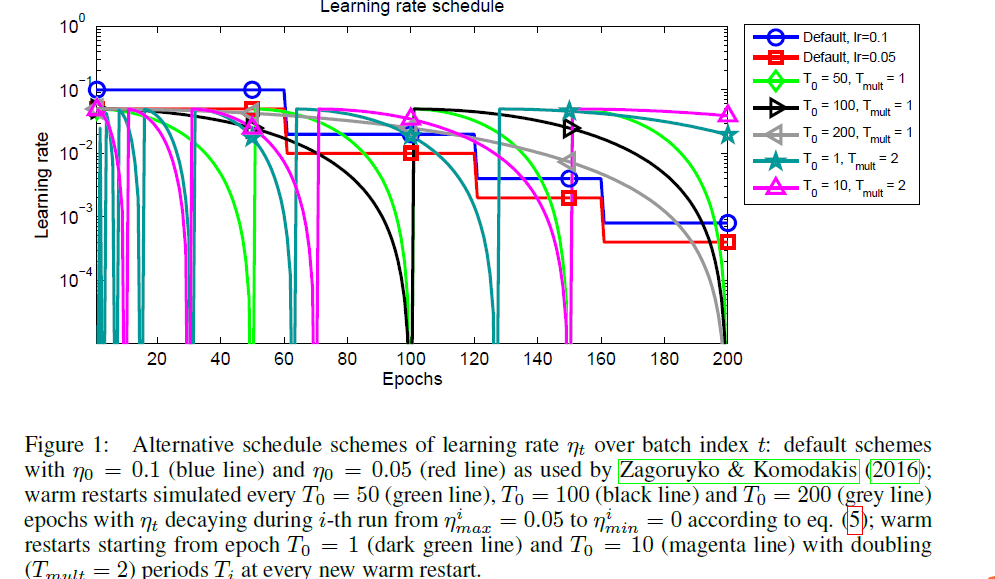
\includegraphics[width=14cm]{SGDR.png}
	%\caption{SGDR}\label{}
\end{figure}

\subsubsection{Experient result in Cifar100}
Init learning rate:0.1\\
Normal augment:ramdom crop and random horizontal flip.\\
\begin{tabular}{| l | c | c | c | c | c | r |}
	\hline
	Augment & Optim & Learning rate & Warm up & Epoch & Train acc & Valid acc \\
	\hline
	FAA   & SGD   & cosine        & Yes     & 3000  & 97.9\%    & 81.6\%\\
	\hline
	Normal   & SGD   & cosine        & Yes     & 3000  & 99.9\%    & 80.3\%\\
	\hline
	Normal   & SGD   & cosine        & No      & 3000  & 99.9\%    & 79.2\%\\
	\hline
\end{tabular}

\subsubsection{Experient result in Linear Constraint ResNet}
All experients use same setup:600epoch, leanring rate:initial value is 0.1 and using cosine method to decrease,warmup,SGD.\\
\begin{tabular}{| l | c | c | c | r |}
	\hline
	Network                            &Augment   & Paper acc &  acc      &  Parameters\\
	\hline
	pre-act ResNet18$(A^{l,i},B^{l,i})$ & Normal   &   74.33\%  & 78.70\%  &   11M\\
	\hline
	pre-act ResNet18$(A^{l,i},B^{l,i})$ &   FAA    &            & 78.30\%  &   11M\\
	\hline
	pre-act ResNet18$(A^l,B^{l,i})$     & Normal   &    74.51\% & 77.69\%  &   8.1M\\
	\hline
	pre-act ResNet18$(A^l,B^{l,i})$     & FAA      &            & 78.92\%  &   8.1M\\
	\hline
	pre-act ResNet34$(A^{l,i},B^{l,i})$ & Normal   &    77.25\% & 78.28\%  &   21M\\
	\hline
	pre-act ResNet34$(A^{l,i},B^{l,i})$ &   FAA    &            & 80.29\%  &   21M\\
	\hline
	pre-act ResNet34$(A^l,B^{l,i})$     & Normal   &   77.40\%  & 79.63\%  &   13M\\
	\hline
	pre-act ResNet34$(A^l,B^{l,i})$     & FAA      &             & 80.53\% &   13M\\
	\hline
\end{tabular}

As can be seen from the above table, the accuracy using normal augmentation methods is higher than the paper, which may be due to multiple epochs and different learning rate methods. Except the pre-act ResNet18$(A^{l,i},B^{l,i})$,using FAA can impove the accuracy, it's doubt that the accuracy of pre-act ResNet18$(A^{l,i},B^{l,i})$, I will do exoerients to verify. In FAA experients, the training accuracy in 600epoch about 0.97, I guess trainning more epoch will get better auuracy.

\subsubsection{wresnet under different augment number}
In wresnet 40*2 network, using cosine learning rate method and initial is 0.1, under different augment method, the probability is 0.5 for every sub-policy. The result in le below table.\\
\begin{tabular}{| l | c | c | c | c | r |}
	\hline
	policy num   & train acc & train+aug acc & test accuracy  &  test+aug acc & test acc drop\\
	\hline
	2          &  99.97   & 99.97       &  75.45         &   74.60            &  0.85\\
	\hline
	4          &  99.97   & 99.88       &  75.30         &   73.73            &  1.57\\
	\hline
	6          &  99.97   & 97.46       &  77.50         &   73.90            &  3.60\\
	\hline
	8          &  99.97   & 97.80       &  77.01         &   73.69            &  3.32\\
	\hline
	25         &  99.96   & 96.83       &  77.11         &   72.96            &  4.15\\
	\hline
	50         &  99.95   & 96.61       &  77.22         &   73.54            &  3.68\\
	\hline
	75         &  99.92   & 96.47       &  76.77         &   73.07            &  3.70\\
	\hline
	100        &  99.96   & 96.52       &  77.13         &   72.32            &  4.81\\
	\hline
	125        &  99.96   & 96.70       &  77.37         &   72.64            &  4.73\\
	\hline
	150        &  99.95   & 96.40       &  77.25         &   73.24            &  4.01\\
	\hline
	175        &  99.96   & 96.49       &  77.72         &   73.19            &  4.53\\
	\hline
	200        &  99.92   & 95.93       &  77.27         &   72.67            &  4.60\\
	\hline
	225        &  99.95   & 96.42       &  77.61         &   72.70            &  4.91\\
	\hline
	250        &  99.96   & 96.56       &  77.04         &   72.81            &  4.23\\
	\hline
	275        &  99.94   & 96.49       &  77.22         &   72.95            &  4.27\\
	\hline
	300        &  99.94   & 96.61       &  77.66         &   73.52            &  4.14\\
	\hline
	325        &  99.94   & 96.36       &  77.27         &   73.27            &  4.00\\
	\hline
	350        &  99.95   & 96.56       &  77.26         &   72.79            &  4.47\\
	\hline
	375        &  99.95   & 96.64       &  77.46         &   72.74            &  4.72\\
	\hline
	400        &  99.95   & 96.49       &  76.78         &   73.02            &  3.66\\
	\hline
	425        &  99.96   & 96.48       &  77.30         &   73.27            &  4.03\\
	\hline
	450        &  99.95   & 96.51       &  77.42         &   73.40            &  4.02\\
	\hline
	475        &  99.95   & 96.42       &  76.66         &   72.81            &  3.85\\
	\hline
	497        &  99.93   & 95.99       &  76.88         &   72.47            &  4.41\\
	\hline
\end{tabular}

I guess cutout is one of the reasons for this, so next I remove cutout for FAA, and do some experients, the result in the below table.\\
\begin{tabular}{| l | c | c | c | c | r |}
	\hline
	policy num   & train acc & train+aug acc & test accuracy  &  test+aug acc & test acc drop\\
	\hline
	1          &  99.98   & 99.97       &  75.21         &   74.77            &  0.44\\
	\hline
	2          &  99.97   & 99.96       &  75.14         &   74.44            &  0.70\\
	\hline
	3          &  99.89   & 99.89       &  75.05         &   73.77            &  1.28\\
	\hline
	4          &  99.88   & 99.88       &  75.26         &   74.10            &  1.16\\
	\hline
	5          &  99.64   & 99.62       &  75.70         &   73.70            &  2.00\\
	\hline
	6          &  97.56   & 97.61       &  76.99         &   73.91            &  3.08\\
	\hline
	7          &  97.72   & 97.86       &  77.59         &   73.89            &  3.70\\
	\hline
	8          &  97.80   & 97.76       &  76.90         &   73.60            &  3.30\\
	\hline
	9          &  96.93   & 96.97       &  77.62         &   72.95            &  4.67\\
	\hline
	10         &  97.16   & 96.98       &  77.90         &   73.32            &  4.58\\
	\hline
	25         &  96.36   & 96.51       &  76.84         &   72.88            &  3.96\\
	\hline
	50         &  96.12   & 95.97       &  77.41         &   73.18            &  4.23\\
	\hline
	75         &  96.57   & 96.70       &  77.02         &   72.95            &  4.07\\
	\hline
	100        &  96.46   & 96.34       &  77.31         &   73.58            &  3.73\\
	\hline
\end{tabular}

We can see that if $N$ is small number, the drop test accuracy is upward trend, but when $N>10$, the trend is vanish.\\

\subsubsection{wresnet under different probability}
Using differenr $p$, the result in below table.\\
\begin{tabular}{| l | c | c | c | c | r |}
	\hline
	p          & train acc & train+aug acc & test accuracy  &  test+aug acc & test acc drop\\
	\hline
	0.0          &  99.97   & 99.97       &  74.78         &   74.11            &   0.67  \\
	\hline
	0.1          &  99.97   & 98.53       &  76.44         &   74.56            &   1.88  \\
	\hline
	0.2          &  99.96   & 97.83       &  76.72         &   73.68            &   3.04  \\
	\hline
	0.3          &  99.96   & 97.35       &  76.75         &   73.92            &   2.83  \\
	\hline
	0.4          &  99.96   & 96.83       &  76.78         &   73.45            &   3.33  \\
	\hline
	0.5          &  99.96   & 96.66       &  77.07         &   72.61            &   4.46  \\
	\hline
	0.6          &  99.95   & 95.91       &  77.29         &   72.75            &   4.54  \\
	\hline
	0.7          &  99.93   & 95.51       &  77.67         &   72.59            &   5.08  \\
	\hline
	0.8          &  99.92   & 95.13       &  77.67         &   72.05            &   5.62  \\
	\hline
	0.9          &  99.91   & 94.27       &  77.68         &   71.25            &   6.43  \\
	\hline
	1.0          &  99.75   & 93.22       &  77.67         &   70.31            &   7.36  \\
	\hline
\end{tabular}

\subsubsection{Use SE block in MgNet}
\subsubsection{SE block}
The structure of the SE building block is depicted in Fig. 1. For any given transformation $F_{tr}$ mapping the input $X$ to the feature maps $U$ where $U \in R^{H*W*C}$,we can construct a corresponding SE block to perform feature recalibration. The features $U$ are first passed through a squeeze operation, which produces a channel descriptor by aggregating feature maps across their spatial dimensions $(H*W)$. The function of this descriptor is to produce an embedding of the global distribution of channel-wise feature responses, allowing information from the global receptive field of the network to be used by
all its layers. The aggregation is followed by an excitation operation, which takes the form of a simple self-gating mechanism that takes the embedding as input and produces a collection of per-channel modulation weights. These weights are applied to the feature maps $U$ to generate the output of the SE block which can be fed directly into subsequent layers of the network.\\
\begin{figure}[H]
	\centering
	% Requires \usepackage{graphicx}
	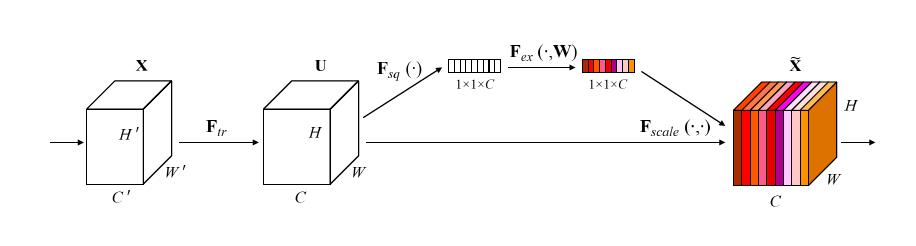
\includegraphics[width=14cm]{seblock.jpg}
	%  %\caption{}\label{}
\end{figure}
Squeeze: Global Information Embedding\\
In order to tackle the issue of exploiting channel dependencies, we first consider the signal to each channel in the output features. Each of the learned filters operates with a local receptive field and consequently each unit of the transformation output $U$ is unable to exploit contextual
information outside of this region. To mitigate this problem, we propose to squeeze global spatial information into a channel descriptor. This is
achieved by using global average pooling to generate channel-wise statistics. Formally, a statistic $z \in R^C$ is generated by shrinking $U$ through its spatial dimensions $H*W$, such that the c-th element of z is calculated by:
\begin{equation}
z_c=F_{sq}(u_c)=\frac{1}{H*W}\sum_{i=1}^H\sum_{j=1}^Wu_c(i,j)
\end{equation}
Excitation: Adaptive Recalibration\\
To make use of the information aggregated in the squeeze operation, we follow it with a second operation which aims to fully capture channel-wise dependencies. To fulfil this objective, the function must meet two criteria: first, it must be flexible (in particular, it must be capable of learning
a nonlinear interaction between channels) and second, it must learn a non-mutually-exclusive relationship since we would like to ensure that multiple channels are allowed to be emphasised (rather than enforcing a one-hot activation). To meet these criteria, we opt to employ a simple gating mechanism with a sigmoid activation:
\begin{equation}
s = F_{ex}(z,W)=\sigma(g(z,W)) = \sigma(W_2\delta(W_1z))
\end{equation}
where $\delta$ refers to the ReLU function,$W_1 \in  R^{\frac{C}{r}*C}$ and$W_2 \in  R^{C*\frac{C}{r}}$. To limit model complexity and aid generalisation, we parameterise the gating mechanism by forming a bottleneck with two fully-connected (FC) layers around the non-linearity, i.e. a dimensionality-reduction layer with reduction ratio $r$, a ReLU and then a dimensionality-increasing layer returning to the channel dimension of the transformation output $U$. The final output of the block is obtained by rescaling $U$ with the activations $s$:
\begin{equation}
x_c = F_{scale}(u_c,s_c) = s_cu_c
\end{equation}
where $X = [x_1,x_2,\dot ,x_C]$and $F_{scale}(u_c,s_c)$ refers to
channel-wise multiplication between the scalar sc and the
feature map $u_c \in R^{H*W}$.


\subsubsection{Add SE block in MgNet}
Modle:MgNet,[2,2,2,2],256 chanels. Add SE block in the end of every Extraction and Restriction block.The result in below table.\\
\begin{tabular}{| l | c | c | c | r |}
	\hline
	Add SE & FAA & epoch & train acc & test acc \\
	\hline
	No     & No  &  300  & 99.95     & 77.64    \\
	\hline
	Yes    & No  &  300  & 99.97     & 78.66    \\
	\hline
	No     & Yes &  300  & 79.36     & 73.65    \\
	\hline
	Yes    & Yes &  300  & 95.95     & 80.17    \\
	\hline
	Yes    & Yes &  500  & 97.87     & 80.96    \\
	\hline
\end{tabular}

New result:\\
\begin{tabular}{| l | c | c | c | r |}
	\hline
	Add SE & FAA & epoch & train acc & test acc \\
	\hline
	No     & No  &  500  & 99.72     & 79.16    \\
	\hline
	Yes    & No  &  500  & 99.68     & 80.04    \\
	\hline
	Yes    &Yes  &  500  & 96.79    &  81.85    \\
	\hline
\end{tabular}

We can conclude that adding SE block in Mgnet will impove trainning accuracy. We only add SE block in the feature space$U$,next,we will test SE block in Image space $F$, and the number of SE block.\\

\subsubsection{Using SOTA tricks in MgNet}
\begin{itemize}
	\item Aim:Using the SOTA tricks in MgNet, and get the best performance in the MgNet.\\
	\item Approch:All the tricks are divided into three methods: data processing, network structure optimization and training algorithm, study the performance of networks with or without every trick, \\
	\item Network:MgNet[2,2,2,2],ResNet-18,pre-act ResNet-18,WResNet40*2\\
	\item Dataset:Cifar100,Cifar10\\
	\item Timetabel:Plan to complete one or two projects a week.
\end{itemize}


\begin{tabular}{| l |  c  | r |}
	\hline
	Dataset             &      Network   &           Train Algorithm\\
	\hline
	Cutout              &       SE       &            \\
	\hline
	Mixup               &       GE       &            \\
	\hline
	Cutmix              &       SK       &             \\
	\hline
	FAA                 &                &             \\
	\hline
\end{tabular}


\begin{figure}[H]
	\centering
	% Requires \usepackage{graphicx}
	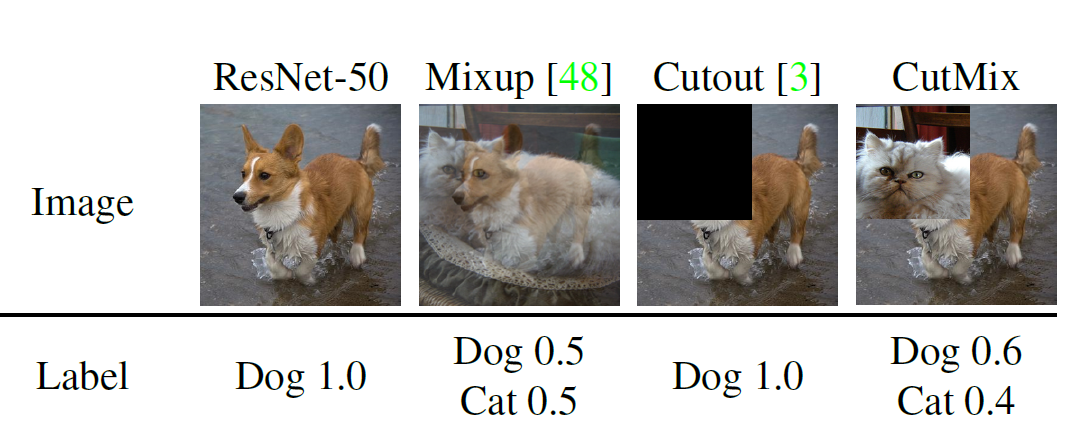
\includegraphics[width=14cm]{dataset-duibi.jpg}
	\caption{Three different dataset augment methods.}\label{Three different dataset augment methods.}
\end{figure}

%\subsubsection{Cutout}
%\begin{figure}[H]
%  \centering
%  % Requires \usepackage{graphicx}
%  \includegraphics[width=13cm]{cutout.jpg}
%%  %\caption{}\label{}
%\end{figure}

\subsubsection{Mixup}
\begin{figure}[H]
	\centering
	% Requires \usepackage{graphicx}
	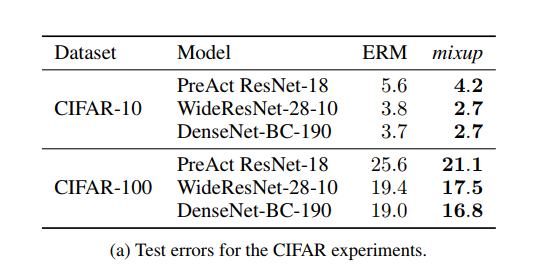
\includegraphics[width=10cm]{mixup.jpg}
	%  %\caption{}\label{}
\end{figure}

\subsubsection{CutMix}
\begin{figure}[H]
	\centering
	% Requires \usepackage{graphicx}
	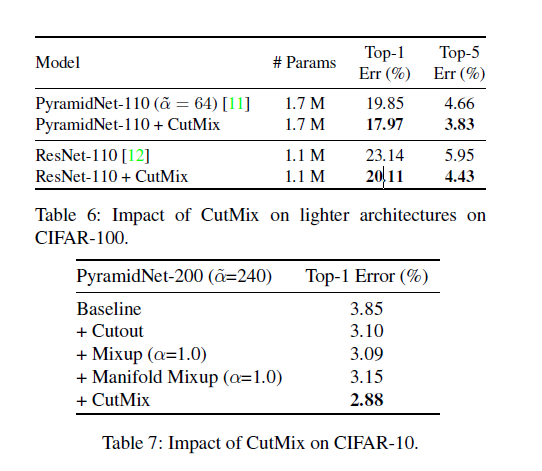
\includegraphics[width=10cm]{cutmix.jpg}
	%  %\caption{}\label{}
\end{figure}

\subsubsection{GE}
\begin{figure}[H]
	\centering
	% Requires \usepackage{graphicx}
	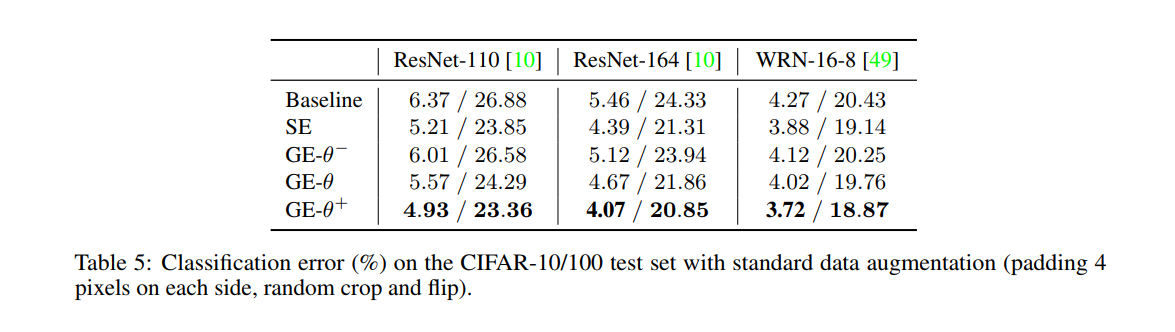
\includegraphics[width=18cm]{GE.png}
	%  %\caption{}\label{}
\end{figure}

\subsubsection{SK}
\begin{figure}[H]
	\centering
	% Requires \usepackage{graphicx}
	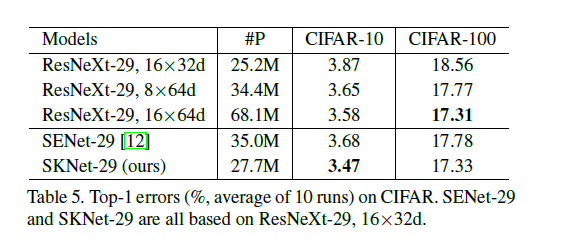
\includegraphics[width=12cm]{SK.jpg}
	%  %\caption{}\label{}
\end{figure}


\newpage
\subsubsection{Add or not add cutout in different models result}
\quad
Table 1:The accuracy in cifar10 for different models.\\
\begin{tabular}{| l | c | c | r |}
	\hline
	Network                &     Parameters   &       paper accuracy   &   my accuracy     \\
	\hline
	ResNet18               &      11.2M      &          95.28         &     94.56          \\
	\hline
	PreActResNet18         &      11.2M      &          94.40         &     94.82          \\
	\hline
	Wide ResNet(40*2)      &      2.2M       &          94.67         &     95.17          \\
	\hline
	Wide ResNet(28*10)     &      36.5M      &          96.12         &     96.06          \\
	\hline
	MgNet[2,2,2,2]-256         &      8.2M       &                        &     96.00          \\
	\hline
	MgNet[3,4,6,3]-256         &      8.3M       &                        &     95.98          \\
	\hline
	MgNet[2,2,2,2]-512         &      33.1M       &                        &               \\
	\hline
\end{tabular}

\vbox{}
Table 2:The accuracy in cifar10 for different models with cutout=16.\\
\begin{tabular}{| l | c | c | r |}
	\hline
	Network                &     Parameters   &       paper accuracy   &   my accuracy     \\
	\hline
	ResNet18               &      11.2M      &          96.01         &     95.19          \\
	\hline
	PreActResNet18         &      11.2M      &                        &     95.74          \\
	\hline
	Wide ResNet(40*2)      &      2.2M       &          95.88         &     95.87          \\
	\hline
	Wide ResNet(28*10)     &      36.5M      &          96.92         &     96.95          \\
	\hline
	MgNet[2,2,2,2]-256         &      8.2M       &                        &     96.89          \\
	\hline
	MgNet[3,4,6,3]-256         &      8.3M       &                        &     96.90          \\
	\hline
	MgNet[2,2,2,2]-512         &      33.1M       &                        &    97.13          \\
	\hline
\end{tabular}


\vbox{}
Table 3:The accuracy in cifar10 for different models with FAA.\\
\begin{tabular}{| l | c | c | r |}
	\hline
	Network                &     Parameters   &       paper accuracy   &   my accuracy     \\
	\hline
	ResNet18               &      11.2M      &                         &      96.46         \\
	\hline
	PreActResNet18         &      11.2M      &                         &                  \\
	\hline
	Wide ResNet(40*2)      &      2.2M       &         96.30           &              \\
	\hline
	Wide ResNet(28*10)     &      36.5M      &         97.30           &               \\
	\hline
	MgNet[2,2,2,2]         &      8.2M       &                         &       97.29         \\
	\hline
	MgNet[3,4,6,3]         &      8.3M       &                         &       97.51          \\
	\hline
	MgNet[2,2,2,2]-512     &      33.1M      &                        &       97.81         \\
	\hline
	MgNet[2,2,2,2]-512,lr:resnet&      33.1M      &              &                \\
	\hline
\end{tabular}

\vbox{}
Table 4:The accuracy in cifar100 for different models.\\
\begin{tabular}{| l | c | c | r |}
	\hline
	Network                &     Parameters   &       paper accuracy   &   my accuracy     \\
	\hline
	ResNet18               &      11.2M      &            77.54       &       76.38(75.38)        \\
	\hline
	PreActResNet18         &      11.2M      &            74.40       &       75.68        \\
	\hline
	Wide ResNet(40*2)      &      2.2M       &            74.00       &              \\
	\hline
	Wide ResNet(28*10)     &      36.5M      &            81.20       &               \\
	\hline
	MgNet[2,2,2,2]-256     &      8.2M       &                        &       79.23         \\
	\hline
	MgNet[3,4,6,3]-256     &      8.3M       &                        &       79.66           \\
	\hline
	MgNet[2,2,2,2]-512     &      33.1M      &                        &       80.43         \\
	\hline
	MgNet[2,2,2,2]-512,lr:resnet &      33.1M      &                        &       81.12         \\
	\hline
	MgNet[3,4,6,3]-512     &      33.1M      &                        &       80.78         \\
	\hline
\end{tabular}

\vbox{}
Table 5:The accuracy in cifar100 for different models with cutout=16.\\
\begin{tabular}{| l | c | c | r |}
	\hline
	Network                &     Parameters   &       paper accuracy   &   my accuracy     \\
	\hline
	ResNet18               &      11.2M      &         78.04           &      76.28         \\
	\hline
	PreActResNet18         &      11.2M      &                         &      76.63         \\
	\hline
	Wide ResNet(40*2)      &      2.2M       &         74.80           &              \\
	\hline
	Wide ResNet(28*10)     &      36.5M      &         81.60           &               \\
	\hline
	MgNet[2,2,2,2]         &      8.2M       &                         &       80.93         \\
	\hline
	MgNet[3,4,6,3]         &      8.3M       &                         &       81.63          \\
	\hline
	MgNet[2,2,2,2]-512     &      33.1M      &                        &       81.83         \\
	\hline
	MgNet[2,2,2,2]-512,lr:resnet  &      33.1M      &                        &                \\
	\hline
\end{tabular}



\vbox{}
Table 6:The accuracy in cifar100 for different models with FAA.\\
\begin{tabular}{| l | c | c | r |}
	\hline
	Network                &     Parameters   &       paper accuracy   &   my accuracy     \\
	\hline
	ResNet18               &      11.2M      &                         &      79.47         \\
	\hline
	PreActResNet18         &      11.2M      &                         &                  \\
	\hline
	Wide ResNet(40*2)      &      2.2M       &         79.40           &              \\
	\hline
	Wide ResNet(28*10)     &      36.5M      &         82.70           &               \\
	\hline
	MgNet[2,2,2,2]-256     &      8.2M       &                         &       82.66         \\
	\hline
	MgNet[3,4,6,3]-256     &      8.3M       &                         &       83.51          \\
	\hline
	MgNet[2,2,2,2]-512     &      33.1M      &                        &       83.75(3)         \\
	\hline
	MgNet[2,2,2,2]-512,lr:resnet&      33.1M      &              &       83.33         \\
	\hline
	MgNet[3,4,6,3]-512     &      33.1M      &              &       84.14         \\
	\hline
\end{tabular}

\vbox{}
Table 7: The accuracy in cifar100 for MgNet with FAA.\\
\begin{tabular}{| l | c | r |}
	\hline
	Network                             &     Parameters   &       accuracy   \\
	\hline
	MgNet[2,2,2,2],[64,128,256,512]     &      9.9M        &        64.36      \\
	\hline
\end{tabular}
\vbox{}


\subsubsection{Multi-step MgNet}
Chebyshev-semi MgNet:\\
\begin{equation}
u^{l,i} = \omega ^{l,i}(u^{l,i-1} + B^{l,i}(f^l - A^l(u^{{l,i-1}}))) + (1 - \omega ^{l,i})u^{l,i-2},i = 1:v_l
\end{equation}

Choose $\omega ^{l,i} = \frac{1}{2}$, the cifar100 results are shown in the table below:\\

\begin{tabular}{| l | c | r |}
	\hline
	Network                  &     Parameters   &       accuracy  \\
	\hline
	MgNet[2,2,2,2],256,C     &      8.3M        &        79.48    \\
	\hline
	MgNet[2,2,2,2],256       &      8.3M        &        79.23    \\
	\hline
	MgNet[3,4,6,3],256,C     &      8.3M        &        80.04    \\
	\hline
	MgNet[3,4,6,3],256       &      8.3M        &        79.66    \\
	\hline
\end{tabular}

\vbox{}
Change Chebyshev-semi MgNet into below formula:\\
\begin{equation}
u^{l,i} = \alpha_1 ^{l,i}(u^{l,i-1} + B^{l,i}(f^l - A^l(u^{{l,i-1}}))) + \alpha_2 ^{l,i}u^{l,i-2},i = 1:v_l
\end{equation}
\vbox{}
$\alpha_1$ and $\alpha_2$ can use trianable parameter or take the definite value.\\

\begin{tabular}{| l | c | c | r |}
	\hline
	$\alpha$ mode &     Network             &     Parameters   &       accuracy   \\
	\hline
	trainable     &    MgNet[4,2,2,2],256   &       8.3M       &        79.43   \\
	\hline
	trainable     &    MgNet[4,4,4,4],256   &       8.3M       &        79.74   \\
	\hline
	trainable     &    MgNet[6,2,2,2],256   &       8.3M       &        79.98 \\
	\hline
	&                         &                  &              \\
	\hline
	0.5           &    MgNet[4,2,2,2],256   &       8.3M       &        80.96 \\
	\hline
	0.5           &    MgNet[4,4,4,4],256   &       8.3M       &        80.87 \\
	\hline
	0.5           &    MgNet[6,2,2,2],256   &       8.3M       &        81.42 \\
	\hline
	0.5           &    MgNet[8,2,2,2],256   &       8.3M       &        81.32 \\
	\hline
	&                         &                  &              \\
	\hline
	1             &    MgNet[4,2,2,2],256   &       8.3M       &        80.99 \\
	\hline
	1             &    MgNet[4,4,4,4],256   &       8.3M       &        79.28 \\
	\hline
	1             &    MgNet[6,2,2,2],256   &       8.3M       &        80.87 \\
	\hline
	1             &    MgNet[8,2,2,2],256   &       8.3M       &        80.50 \\
	\hline
\end{tabular}

\vbox{}
Multi-step MgNet:\\
\begin{equation}
u^{l,i} = \sum _{j=0}^{i-1}\alpha _j^{l,i}(u^{l,j} + B_j^{l,i}(f^l-A^l(u^{l,j}))),i = 1:v_l
\end{equation}

\begin{equation}
u^{l,i} = \alpha_1(u^{l,i-1}+B^{l,i-1}(f^l-A^l(u^{l,j}))) + \alpha_2\sum _{j=0}^{i-2}(u^{l,j} + B_j^{l,i}(f^l-A^l(u^{l,j}))),i = 1:v_l
\end{equation}

\vbox{}
choose $\alpha_1=\alpha_2=0.5$, have below result:\\

\begin{tabular}{| l | c | r |}
	\hline
	Network                  &     Parameters   &       accuracy   \\
	\hline
	MgNet[2,2,2,2],256     &      8.3M          &        79.94       \\
	\hline
	MgNet[4,2,2,2],256     &      8.3M          &        80.24       \\
	\hline
	MgNet[4,4,4,4],256     &      8.3M          &        80.38      \\
	\hline
	MgNet[6,2,2,2],256     &      8.3M          &        80.27       \\
	\hline
\end{tabular}

\vbox{}
choose $\alpha_1=\alpha_2=1$, have below result:\\
\begin{tabular}{| l | c | r |}
	\hline
	Network                &     Parameters     &       accuracy   \\
	\hline
	MgNet[2,2,2,2],256     &      8.3M          &        78.86       \\
	\hline
	MgNet[4,2,2,2],256     &      8.3M          &        79.72       \\
	\hline
	MgNet[6,2,2,2],256     &      8.3M          &        79.67       \\
	\hline
	MgNet[8,2,2,2],256     &      8.3M          &        79.45       \\
	\hline
\end{tabular}

\vbox{}
choose $\alpha_1=\alpha_2=trainable$, have below result:\\
\begin{tabular}{| l | c | r |}
	\hline
	Network                &     Parameters     &       accuracy   \\
	\hline
	MgNet[2,2,2,2],256     &      8.3M          &        76.52       \\
	\hline
	MgNet[4,2,2,2],256     &      8.3M          &        79.90       \\
	\hline
	MgNet[6,2,2,2],256     &      8.3M          &        80.40       \\
	\hline
	MgNet[8,2,2,2],256     &      8.3M          &               \\
	\hline
\end{tabular}

\vbox{}
choose $\alpha_1=1,\alpha_2=trainable$, have below result:\\
\begin{tabular}{| l | c | r |}
	\hline
	Network                &     Parameters     &       accuracy   \\
	\hline
	MgNet[2,2,2,2],256     &      8.3M          &        79.32       \\
	\hline
	MgNet[4,2,2,2],256     &      8.3M          &        79.89       \\
	\hline
	MgNet[6,2,2,2],256     &      8.3M          &                    \\
	\hline
	MgNet[8,2,2,2],256     &      8.3M          &                    \\
	\hline
\end{tabular}

\subsubsection{Retrieval DenseNet in cifar100 result}
\begin{tabular}{| l   | c | c  | r |}
	\hline
	Network                  &     Parameters   &       my accuracy  & paper accuracy   \\
	\hline
	DenseNet(k=12,100)       &     0.8M         &       76.91        & 77.63 \\
	\hline
	DenseNet(k=24,250)       &     15.3M         &      81.03        & 82.40 \\
	\hline
\end{tabular}

\subsubsection{Increasing the number of channels in MgNet }
In the previous , the number of channels in MgNet is a fixed value, such as 256,this will greatly increase the parameters of the first module. In this seceion, we will increasing channel number in each MgNet block.\\
\vbox{}
\begin{tabular}{| l | c | r |}
	\hline
	Network                  &     Parameters   &       accuracy   \\
	\hline
	MgNet[2,2,2,2]           &      9.4M        &      79.28  \\
	\hline
	MgNet[4,2,2,2]           &      9.4M        &      79.27  \\
	\hline
	MgNet[6,2,2,2]           &      9.4M        &      79.71  \\
	\hline
	MgNet[10,2,2,2]          &      9.4M        &      78.52  \\
	\hline
	MgNet[4,4,4,4]           &      9.4M        &      78.32  \\
	\hline
	MgNet[3,4,6,3]           &      9.4M        &      78.30  \\
	\hline
	MgNet[2,2,2,6]           &      9.4M        &      77.87  \\
	\hline
\end{tabular}

\newpage
\section{MgNet test in Imagenet}

\begin{table}[H]
	\begin{tabular}{| l | c | c | c | c | c | r |}
		\hline
		model          &   num ite                 &      channels          &     paras   &   epoch      &    last  acc  &  max  acc \\
		\hline
		%MgNet          &   3,3,5,2(wise-B)         &  [64,128,256,512]      &   14.98M    &  160         &    74.98      & 75.13     \\
		%\hline
		%MgNet          &   3,4,6,3(wise-B)         &  [64,128,256,512]      &   18.08M    &  160         &    75.63      & 75.73     \\
		%\hline
		%MgNet          &   2,2,2,2(not wise-B)     &  [128,256,512,1024]    &   38.52M    &  160         &    76.74      & 76.82     \\
		%\hline
		%MgNet          &   2,2,2,2(wise-B)         &  [128,256,512,1024]    &   51.05M    &  160         &    77.17      & 77.27     \\
		%\hline
		%MgNet          &   2,2,4,2(not wise-B)     &  [128,256,512,1024]    &   38.52M    &  160         &    77.41      & 77.58     \\
		%\hline
		%MgNet          &   2,2,4,2(wise-B)         &  [128,256,512,1024]    &   55.77M    &  160         &    77.89      & 77.94     \\
		%\hline
		DenseNet-121   &   6,12,24,16              &  -                     &     9M      &              &    -          & 74.98     \\
		\hline
		DenseNet-169   &   6,12,32,32              &  -                     &     14M     &              &    -          & 76.20     \\
		\hline
		DenseNet-201   &   6,12,48,32              &  -                     &     20M     &              &    -          & 77.42     \\
		\hline
		DenseNet-264   &   6,12,64,48              &  -                     &     33M     &              &    -          & 77.85     \\
		\hline
	\end{tabular}
\end{table}
\subsection{Huang Huang's results}
\subsubsection{Fix channel in MgNet}
\begin{table}[H]
	\begin{tabular}{| l | c | c | c | r |}
		\hline
		num ite    &      channels      &    Parameters   &   last accuracy   &  best accuracy  \\
		\hline
		[2,2,2,2]   &         256        &    8.5M         &   70.83           &  71.01          \\
		\hline
	\end{tabular}
\end{table}

\subsubsection{Increase channel in MgNet}
\begin{table}[H]
	\begin{tabular}{| l | c | c | c | r |}
		\hline
		num ite    &      channels      &    Parameters   &   last accuracy   &  best accuracy  \\
		\hline
		[2,2,2,2]   &  [64,128,256,512]  &    9.9M         &   72.32           &  72.32          \\
		\hline
		[2,2,4,2]   &  [64,128,256,512]  &    9.9M         &   73.04           &  73.04          \\
		\hline
		[2,2,8,2]   &  [64,128,256,512]  &    9.9M         &   73.66           &  73.72          \\
		\hline
		[2,2,16,2]  &  [64,128,256,512]  &    9.9M         &   73.74           &  73.81          \\
		\hline
		\hline
		[3,3,5,2]   &  [64,128,256,512]  &    9.9M         &   73.39           &  73.47          \\
		\hline
		[3,4,6,3]   &  [64,128,256,512]  &    9.9M         &   73.69           &  73.78          \\
		\hline
		\hline
		[2,2,2,2]   & [128,256,512,1024] &   38.5M         &   76.75           &  76.82          \\
		\hline
		[2,2,4,2]   & [128,256,512,1024] &   38.5M         &   77.41           &  77.58           \\
		\hline
	\end{tabular}
\end{table}

\subsection{Jianqing's results}
\subsection{Increase channel in MgNet with wise-B}
\begin{table}[H]
	\begin{tabular}{| l | c | c | c | r |}
		\hline
		num ite    &      channels      &    Parameters   &   last accuracy   &  best accuracy  \\
		\hline
		[2,2,2,2]   &  [64,128,256,512]  &    13.0M         &   73.24           &  73.36          \\
		\hline
		[4,2,2,2]   &  [64,128,256,512]  &    13.1M         &   73.48           &  73.56          \\
		\hline
		[3,3,5,2]   &  [64,128,256,512]  &    15.4M         &   74.46           &  74.54          \\
		\hline
		[3,4,6,3]   &  [64,128,256,512]  &    18.1M         &   75.23           &  75.23          \\
		\hline
		[2,2,4,2]   &  [64,128,256,512]  &    14.7M         &   74.37           &  74.58          \\
		\hline
		[2,2,8,2]   &  [64,128,256,512]  &    16.6M         &   75.16           &  75.18          \\
		\hline
		\hline
		[2,2,2,2]   &  [128,256,512,1024]    &   51.1M     &    77.17          & 77.27     \\
		\hline
		[2,2,4,2]   &  [128,256,512,1024]    &   55.7M     &    77.89          & 77.94     \\
		\hline
		[3,4,6,3]   &  [128,256,512,1024]    &   66.7M     &                   & 78.65     \\
		\hline
	\end{tabular}
\end{table}

\newpage
\section{MgNet test in Cifar100}

\subsection{The DenseNet Classification Results on CIFAR}
\begin{tabular}{| l | c | c | c  | c | c | r |}
	\hline
	Method              &   Depth   & Params   & C10    & C10+    & C100   &   C100+ \\
	\hline
	Densenet(k=12)      &    40     & 1.0M     & 93.00  & 94.76   & 72.45  &   75.58  \\
	\hline
	Densenet(k=12)      &   100     & 7.0M     & 94.23  & 95.90   & 76.21  &   79.80  \\
	\hline
	Densenet(k=24)      &   100     & 27.2M    & 94.17  & 96.26   & 76.58  &   80.75  \\
	\hline
	Densenet-BC(k=12)   &   100     & 0.8M     & 94.08  & 95.49   & 75.85  &   77.73  \\
	\hline
	Densenet-BC(k=24)   &   250     & 15.3M    & 94.81  & 96.38   & 80.36  &   82.40  \\
	\hline
	Densenet-BC(k=40)   &   190     & 25.6M    & -      & 96.54   & -      &   82.72  \\
	\hline
\end{tabular}
\\ \hspace*{\fill} \\
Refer the DenseNet with $\alpha<1$ as DenseNet-C, and  set $\alpha=0.5$in experiment.When both the bottleneck and transition layers with $\alpha<1$
are used, refer  as DenseNet-BC.\\
$'+'$ indicates standard data augmentation.

\subsection{Huang Huang's result}
\begin{table}[H]
	\begin{tabular}{| l | c | c | c | c | r |}
		\hline
		num ite       &      channels           &    Parameters   &   last accuracy   &  best accuracy  \\
		\hline
		[2,2,2,2]      & [64,128,256,512]        &    9.43M        &    78.22          &  78.25          \\
		\hline
		[4,2,2,2]      & [64,128,256,512]        &    9.43M        &    78.33          &  78.52          \\
		\hline
		[8,2,2,2]      & [64,128,256,512]        &    9.43M        &    78.29          &  78.42          \\
		\hline
		[16,2,2,2]     & [64,128,256,512]        &    9.43M        &    78.13          &  78.25          \\
		\hline
		[32,2,2,2]     & [64,128,256,512]        &    9.43M        &    78.69          &  78.80          \\
		\hline
		[4,4,4,4]      & [64,128,256,512]        &    9.43M        &    77.89          &  77.99          \\
		\hline
		[3,3,5,2]      & [64,128,256,512]        &    9.43M        &    78.38          &  78.54          \\
		\hline
		[2,8,2,2]      & [64,128,256,512]        &    9.43M        &    78.53          &  78.68          \\
		\hline
		[2,2,8,2]      & [64,128,256,512]        &    9.43M        &    78.38          &  78.70          \\
		\hline
		[2,8,8,2]      & [64,128,256,512]        &    9.44M        &    78.33          &  78.44          \\
		\hline
		[2,2,16,2]     & [64,128,256,512]        &    9.44M        &    78.77          &  78.95          \\
		\hline
		[2,16,2,2]     & [64,128,256,512]        &    9.43M        &    78.42          &  78.52          \\
		\hline
		[2,2,32,2]     & [64,128,256,512]        &    9.45M        &    78.48          &  78.67          \\
		\hline
	\end{tabular}
\end{table}

\subsection{Jianqing's result}
\subsubsection{Increase channel in MgNet}
\begin{table}[H]
	\begin{tabular}{| l | c | c | c | c | r |}
		\hline
		num ite       &      channels        &  trick     &    Parameters   &   last accuracy   &  best accuracy  \\
		\hline
		[2,2,2,2]      & [64,128,256,512]     &  wise B    &    12.2M        &    78.57          &  78.86          \\
		\hline
		[4,2,2,2]      & [64,128,256,512]     &  wise B    &    12.5M        &    79.01          &  79.23          \\
		\hline
		[8,2,2,2]      & [64,128,256,512]     &  wise B    &    12.8M        &    79.44          &  79.55          \\
		\hline
		[16,2,2,2]     & [64,128,256,512]     &  wise B    &    13.1M        &    80.05          &  80.39          \\
		\hline
		[24,2,2,2]     & [64,128,256,512]     &  wise B    &    13.4M        &    80.52          &  80.52          \\
		\hline
		\hline
		[2,2,8,2]      & [64,128,256,512]     &  wise B    &    16.1M        &    80.20          &  80.24          \\
		\hline
		[2,2,16,2]     & [64,128,256,512]     &  wise B    &    20.8M        &    79.83          &  80.03          \\
		\hline
		\hline
		[4,4,4,4]      & [64,128,256,512]     &  wise B    &    18.8M        &    78.42          &  78.80          \\
		\hline
		[6,6,6,6]      & [64,128,256,512]     &  wise B    &    25.1M        &    78.73          &  78.84          \\
		\hline
		[8,8,8,8]      & [64,128,256,512]     &  wise B    &    31.4M        &    79.09          &  79.10          \\
		\hline
	\end{tabular}
\end{table}



\subsubsection{Fix channel in MgNet}
\begin{table}[H]
	\begin{tabular}{| l | c | c | c | c | r |}
		\hline
		num ite       &      channels        &  trick     &    Parameters   &   last accuracy   &  best accuracy  \\
		\hline
		[4,2,2,2]      &      256             &  wise-B    &    11.9M        &       80.48       &  80.63          \\
		\hline
		[6,2,2,2]      &      256             &  wise-B    &    13.1M        &       80.94       &  81.11          \\
		\hline
		[8,2,2,2]      &      256             &  wise-B    &    14.3M        &       81.42       &  81.42          \\
		\hline
		\hline
		[4,2,2,2]      &      256             &  csbv,wise-B      &    11.9M         &       81.30       &  81.32         \\
		\hline
		[6,2,2,2]      &      256             &  csbv,wise-B      &    13.1M         &       81.08       &  81.33          \\
		\hline
		[8,2,2,2]      &      256             &  csbv,wise-B      &    14.3M         &       81.21       &  81.32          \\
		\hline
		[16,2,2,2]     &      256             &  csbv,wise-B      &    18.9M         &       81.18       &  81.19          \\
		\hline
		\hline
		[3,4,6,3]      &      256             &  csbv,wise-B      &    15.4M         &       81.05       &  81.15          \\
		\hline
	\end{tabular}
\end{table}

\subsubsection{Architecture from ResNet}
In ResNet and DenseNet cifar experiments, the networks have three mesh size and in every mesh size have the same number blocks(layers), use this method for design MgNet networks.
\begin{table}[H]
	\begin{tabular}{| l | c | c | c | c | r |}
		\hline
		num ite       &      channels        &  wise-B     &    Parameters   &   last accuracy   &  best accuracy  \\
		\hline
		[2,2,2]        &   [128,256,512]      &  No         &    9.2M         &    79.37          &  79.42          \\
		\hline
		[4,4,4]        &   [128,256,512]      &  No         &    9.2M         &    79.74          &  79.85          \\
		\hline
		[6,6,6]        &   [128,256,512]      &  No         &    9.2M         &    79.01          &  79.01          \\
		\hline
		[8,8,8]        &   [128,256,512]      &  No         &    9.2M         &    78.45          &  78.51          \\
		\hline
		\hline
		[2,2,2]        &   [128,256,512]      &  Yes        &    12.3M        &    79.82          &  79.92          \\
		\hline
		[4,4,4]        &   [128,256,512]      &  Yes        &    18.5M        &    81.27          &  81.27          \\
		\hline
		[6,6,6]        &   [128,256,512]      &  Yes        &    24.7M        &    80.53          &  80.69          \\
		\hline
		[8,8,8]        &   [128,256,512]      &  Yes        &    30.9M        &    80.17          &  80.36          \\
		\hline
		\hline
		[10,10,4]      &   [128,256,512]      &  Yes        &    22.9M        &    80.86          &  80.96          \\
		\hline
		[12,12,4]      &   [128,256,512]      &  Yes        &    24.4M        &    80.55          &  80.90          \\
		\hline
	\end{tabular}
\end{table}

\subsubsection{Bottleneck}
In this part, I designed the bottleleck of MgNet in the same way as ResNet, the restriction as below:
\begin{equation}
u^{\ell,i} = u^{\ell,i-1} + C^{\ell}B^{\ell,i}  (f^\ell -  A^{\ell} (u^{\ell,i-1})).
\end{equation}
and $A^{\ell},C^{\ell}\in \mathbb{R}^{c\times c\times 3\times 3},\quad B^{\ell,i}\in \mathbb{R}^{c\times c\times 1\times 1}$

\begin{table}[H]
	\begin{tabular}{| l | c | c | c | c | r |}
		\hline
		num ite       &      channels        &  wise-B     &    Parameters   &   last accuracy   &  best accuracy  \\
		\hline
		[2,2,2]        &   [128,256,512]      &  No         &    9.5M         &    78.54          &  78.64          \\
		\hline
		[4,4,4]        &   [128,256,512]      &  No         &    9.5M         &    78.49          &  78.55          \\
		\hline
		[6,6,6]        &   [128,256,512]      &  No         &    9.6M         &    78.03          &  78.35          \\
		\hline
		[8,8,8]        &   [128,256,512]      &  No         &    9.6M         &    77.69          &  77.73          \\
		\hline
		\hline
		[2,2,2]        &   [128,256,512]      &  Yes        &    9.9M         &    78.78          &  78.92          \\
		\hline
		[4,4,4]        &   [128,256,512]      &  Yes        &    10.6M        &    79.10          &  79.42          \\
		\hline
		[6,6,6]        &   [128,256,512]      &  Yes        &    11.3M        &    79.46          &  79.61          \\
		\hline
		[8,8,8]        &   [128,256,512]      &  Yes        &    12.0M        &    76.27          &  76.45          \\
		\hline
	\end{tabular}
\end{table}

\subsubsection{Bottleneck-Juncai}
In this part, Juncai He designed the bottleleck of MgNet as below:
\begin{equation}
u^{\ell,i} = u^{\ell,i-1} + P^{\ell,i}B^{\ell,i}Q^{\ell,i}(f^\ell -  A^{\ell} (u^{\ell,i-1})).
\end{equation}
and $A^{\ell},B^{\ell,i}\in \mathbb{R}^{c_{in}\times c_{out}\times 3\times 3},\quad P^{\ell,i},Q^{\ell,i} \in \mathbb{R}^{c_{in}\times c_{out}\times 1\times 1}$

\begin{table}[H]
	\begin{tabular}{| l | c | c | c | c | r |}
		\hline
		num ite       &      channels        &  wise-B     &    Parameters   &   last accuracy   &  best accuracy  \\
		\hline
		[6,6,6]        &   [128,256,512]      &  Yes        &    8.3M         &      78.81        &    78.81        \\
		\hline
		[8,8,8]        &   [128,256,512]      &  Yes        &    9.1M         &      77.97        &    77.97        \\
		\hline
		\hline
		[3,4,6,3]      & [64,128,256,512]     &  Yes        &    7.6M         &      76.64       &    76.64        \\
		\hline
		[3,4,8,3]      & [64,128,256,512]     &  Yes        &    7.8M         &      76.58       &    76.86        \\
		\hline
		[3,4,12,3]     & [64,128,256,512]     &  Yes        &    8.1M         &      76.68       &    77.01        \\
		\hline
		\hline
		[3,4,6,3]      & [128,256,512,1024]   &  Yes        &    30.4M        &      79.13       &    79.29        \\
		\hline
		[3,4,8,3]      & [128,256,512,1024]   &  Yes        &    30.9M        &      79.57       &    79.57        \\
		\hline
		[3,4,12,3]     & [128,256,512,1024]   &  Yes        &    32.1M        &      78.45       &    78.80        \\
		\hline
	\end{tabular}
\end{table}



\newpage
\subsection{MgNet Summary}
\subsubsection{Comprision of  fixed channels version MgNet  and increase channels version MgNet}
\begin{enumerate}
\item In cifar100, fixed channels accuracy higher than increase channels.
\begin{table}[!htbp]
	%\caption{MgNet: $B^{\ell,i}=\sigma \circ \eta^{\ell} \circ \sigma,\quad c_\ell=c_1$}
	%\label{tabel:mgnet-1}
	\begin{center}

		\begin{tabular}{|c|c|c|c|c|}
			\hline
			$[\nu_1,\nu_2,\cdots,\nu_J], c_\ell$,   &  test accuracy
			& parameters   \tabularnewline
			\hline
			[2,2,2,2], 256    &  79.94(79.67)  & 8.3M
			\tabularnewline
			\hline			
			[2,2,2,2],512     & 81.35(81.12)     & 33.1M
			\tabularnewline
			\hline
			[2,2,2,2],768     & 81.74(81.67)     & 74.4M
			\tabularnewline
			\hline
			[2,2,2,2],1024    & 81.89(81.58)   & 132.2M
			\tabularnewline
			\hline						
		\end{tabular}
		%	}
	\end{center}
\end{table}

\begin{table}[!htbp]
	%\caption{MgNet: $B^{\ell,i}=\sigma \circ \eta^{\ell} \circ \sigma$, increase$c_\ell$}
	%\label{tabel:mgnet-2}
	\begin{center}
		%	\resizebox{\textwidth}{!}{
		\begin{tabular}{|c|c|c|c|c|}
			\hline
			$[\nu_1,\nu_2,\cdots,\nu_J], c_\ell$,  &  test accuracy
			& parameters  \tabularnewline
			\hline
			[2,2,2,2], [32,64,128,256]   &  74.95(74.75)  & 2.3M
			\tabularnewline
			\hline			
			[2,2,2,2], [64,128,256,512]      & 78.06(78.04)     & 12.5M
			\tabularnewline
			\hline
			[2,2,2,2],[128,256,512,1024]     & 80.29(80.28)      & 37.5M
			\tabularnewline
			\hline
			[2,2,2,2],[256,512,1024,2048]     & 81.49(81.41)    & 150.0M
			\tabularnewline
			\hline						
		\end{tabular}
		%	}
	\end{center}
\end{table}




\item In ImageNet, increase channels higher than fixed channels accuracy.
\begin{table}[!htbp]
    \begin{center}
        \begin{tabular}{| l | c | c | c | r |}
        \hline
        $[\nu_1,\nu_2,\cdots,\nu_J], c_\ell$,  &  test accuracy & parameters
        \tabularnewline
        \hline
        [2,2,2,2],256                           &    70.83(71.01)&     8.5M
        \tabularnewline
        \hline
        \end{tabular}
     \end{center}
\end{table}

\begin{table}[!htbp]
    \begin{center}
        \begin{tabular}{| l | c | c | c | r |}
        \hline
        $[\nu_1,\nu_2,\cdots,\nu_J], c_\ell$,  &  test accuracy & parameters
        \tabularnewline
        \hline
        [2,2,2,2],[64,128,256,512]             &   72.32(72.32) &   9.9M
        \tabularnewline
        \hline
        \end{tabular}
    \end{center}
\end{table}

\end{enumerate}


\subsubsection{Increase channels in MgNet}
\begin{enumerate}
\item In cifar100, increase channels in fix channels  version MgNet will increase accuracy.
\begin{table}[!htbp]
	%\caption{MgNet: increase $c_\ell$  with $\nu=[2,2,2,2]$}
	%\label{raw MgNet results 1-256 }
	\begin{center}
			\begin{tabular}{|c|c|c|c|}
				\hline
				$[\nu_1,\nu_2,\cdots,\nu_J], c_\ell$,  &  accuracy  best(last) & mgnet parameters \tabularnewline
                \hline
				[2,2,2,2], 256                         &  79.94(79.67)         & 8.3M             \tabularnewline
                \hline
				[2,2,2,2], 512                         &  81.35(81.12)         & 33.1M            \tabularnewline
                \hline
				[2,2,2,2], 1024                        &  81.89(81.58)          & 132.2            \tabularnewline
				\hline
			\end{tabular}
	\end{center}
\end{table}

\begin{table}[!htbp]
	%\caption{MgNet: increase $c_\ell$  with $\nu=[4,2,2,2]$}
	%\label{raw MgNet results 1-256 }
	\begin{center}
			\begin{tabular}{|c|c|c|c|}
				\hline
				$[\nu_1,\nu_2,\cdots,\nu_J], c_\ell$,  &  accuracy  best(last) & mgnet parameters \tabularnewline
                \hline
				[4,2,2,2], 256                         &  80.25(80.02)         & 8.3M             \tabularnewline
                \hline
				[4,2,2,2], 512                         &  81.53(81.25)         & 33.1M            \tabularnewline
				\hline
			\end{tabular}
	\end{center}
\end{table}


\begin{table}[!htbp]
	%\caption{MgNet: increase $c_\ell$  with $\nu=[8,2,2,2]$}
	%\label{raw MgNet results 1-256 }
	\begin{center}
			\begin{tabular}{|c|c|c|c|}
				\hline
				$[\nu_1,\nu_2,\cdots,\nu_J], c_\ell$,  &  accuracy  best(last) & mgnet parameters \tabularnewline
                \hline
				[8,2,2,2], 256                         &  80.32(80.12)         & 8.3M             \tabularnewline
                \hline
				[8,2,2,2], 512                         &  81.83(81.59)         & 33.1M            \tabularnewline
                \hline
				[8,2,2,2], 1024                        &  82.46(82.20)         & 132.2M           \tabularnewline
				\hline
			\end{tabular}
	\end{center}
\end{table}


\newpage
\item In ImageNet, increase channels in increase channels version MgNet will increase accuracy.
\begin{table}[!htbp]
	%\caption{MgNet: increase $c_\ell$  with $\nu=[2,2,2,2]$}
	%\label{raw MgNet results 1-256 }
	\begin{center}
			\begin{tabular}{|c|c|c|c|}
				\hline
				$[\nu_1,\nu_2,\cdots,\nu_J], c_\ell$,  &  accuracy  best(last) & mgnet parameters \tabularnewline
                \hline
				[2,2,2,2], [64,128,256,512]            &  72.32(72.32)         & 9.9M             \tabularnewline
                \hline
				[2,2,2,2], [128,256,512,1024]          &  76.82(76.75)         & 38.5             \tabularnewline
				\hline
			\end{tabular}
	\end{center}
\end{table}

\begin{table}[!htbp]
	%\caption{MgNet: increase $c_\ell$  with $\nu=[2,2,2,2]$}
	%\label{raw MgNet results 1-256 }
	\begin{center}
			\begin{tabular}{|c|c|c|c|}
				\hline
				$[\nu_1,\nu_2,\cdots,\nu_J], c_\ell$,  &  accuracy  best(last) & mgnet parameters \tabularnewline
                \hline
				[2,2,4,2], [64,128,256,512]            &  73.04(73.04)         & 9.9M             \tabularnewline
                \hline
				[2,2,4,2], [128,256,512,1024]          &  77.58(77.41)         & 38.5M             \tabularnewline
				\hline
			\end{tabular}
	\end{center}
\end{table}


\begin{table}[!htbp]
	%\caption{MgNet: increase $c_\ell$  with $\nu=[2,2,2,2]$}
	%\label{raw MgNet results 1-256 }
	\begin{center}
			\begin{tabular}{|c|c|c|c|}
				\hline
				$[\nu_1,\nu_2,\cdots,\nu_J], c_\ell$,  &  accuracy  best(last) & mgnet parameters \tabularnewline
                \hline
				[2,2,2,2], [64,128,256,512](wise-B)    &  73.36(73.24)         & 13.0M             \tabularnewline
                \hline
				[2,2,2,2], [128,256,512,1024](wise-B)  &  77.27(77.17)         & 51.1M             \tabularnewline
				\hline
			\end{tabular}
	\end{center}
\end{table}


\begin{table}[!htbp]
	%\caption{MgNet: increase $c_\ell$  with $\nu=[2,2,2,2]$}
	%\label{raw MgNet results 1-256 }
	\begin{center}
			\begin{tabular}{|c|c|c|c|}
				\hline
				$[\nu_1,\nu_2,\cdots,\nu_J], c_\ell$,  &  accuracy  best(last) & mgnet parameters \tabularnewline
                \hline
				[2,2,4,2], [64,128,256,512](wise-B)    &  74.58(74.37)         & 14.7M             \tabularnewline
                \hline
				[2,2,4,2], [128,256,512,1024](wise-B)  &  77.94(77.89)         & 55.7M             \tabularnewline
				\hline
			\end{tabular}
	\end{center}
\end{table}
\end{enumerate}




\newpage
\subsubsection{Increase $\nu$}
\begin{enumerate}
\item In cifar100, increase $\nu_1$ in fix channels MgNet will increase accuracy.
\begin{table}[!htbp]
	%\caption{MgNet: increase $\nu_1$  with $c_\ell=256$}
	%\label{raw MgNet results 1-256 }
	\begin{center}
			\begin{tabular}{|c|c|c|c|}
				\hline
				$[\nu_1,\nu_2,\cdots,\nu_J], c_\ell$,  &  accuracy  best(last) & mgnet parameters \tabularnewline
				\hline
				[2,2,2,2], 256                         &  79.94(79.67)         & 8.3M             \tabularnewline
				\hline		
				[4,2,2,2], 256                         &  80.25(80.02)         & 8.3M             \tabularnewline
				\hline
				[8,2,2,2], 256                         &  80.32(80.12)         & 8.3M             \tabularnewline
				\hline
				[16,2,2,2], 256                        &  80.42(80.22)         & 8.3M             \tabularnewline
				\hline
				[32,2,2,2], 256                        &  80.89(80.65)         & 8.3M             \tabularnewline
				\hline
			\end{tabular}
	\end{center}
\end{table}


\begin{table}[!htbp]
	%\caption{MgNet: increase $\nu_1$  with $c_\ell=512$}
	%\label{raw MgNet results 1-512 }
	\begin{center}
			\begin{tabular}{|c|c|c|c|}
				\hline
				$[\nu_1,\nu_2,\cdots,\nu_J], c_\ell$,  &   accuracy  best(last) & mgnet parameters \tabularnewline
				\hline
				[2,2,2,2], 512                         &   81.35(81.12)         & 33.1M            \tabularnewline
				\hline
				[4,2,2,2], 512                         &   81.53(81.25)         & 33.1M            \tabularnewline
				\hline
				[8,2,2,2], 512                         &   81.83(81.59)         & 33.1M            \tabularnewline
				\hline
				[16,2,2,2], 512                        &   81.97(81.58)         & 33.1M            \tabularnewline
				\hline
			\end{tabular}
	\end{center}
\end{table}

\begin{table}[!htbp]
	%\caption{MgNet: increase $\nu_1$  with $c_\ell=1024$}
	%\label{raw MgNet results 1-1024 }
	\begin{center}
			\begin{tabular}{|c|c|c|c|}
				\hline
				$[\nu_1,\nu_2,\cdots,\nu_J], c_\ell$,  &  accuracy  best(last)   & mgnet parameters \tabularnewline
				\hline
				[2,2,2,2], 1024                        &   81.89(81.58)          & 132.2            \tabularnewline
				\hline
				[8,2,2,2], 1024                        &   82.46(82.20)          & 132.2            \tabularnewline
				\hline
			\end{tabular}
	\end{center}
\end{table}

\newpage
\item In cifar100, increase $\nu_2$,$\nu_3$,$\nu_4$ the effect is not obvious in fix channels MgNet.
\begin{table}[!htbp]
	%\caption{MgNet: increase $\nu_2$}
	%\label{raw MgNet results 2 }
	\begin{center}
		%\resizebox{\textwidth}{!}{
			\begin{tabular}{|c|c|c|c|}
				\hline
				$[\nu_1,\nu_2,\cdots,\nu_J], c_\ell$   &  accuracy best(last)  & mgnet parameters \tabularnewline
				\hline
				[2,2,2,2], 256                         &  79.94(79.67)         &     8.3M         \tabularnewline
				\hline		
				[2,4,2,2], 256                         &  79.96(79.65)         &     8.3M         \tabularnewline
				\hline
				[2,8,2,2], 256                         &  79.92(79.71)         &     8.3M         \tabularnewline
				\hline
				[2,16,2,2], 256                        &  79.97(79.66)         &     8.3M         \tabularnewline
				\hline
			\end{tabular}
		%}
	\end{center}
\end{table}


\begin{table}[!htbp]
	%\caption{MgNet: increase $\nu_3$}
	%\label{raw MgNet results 3 }
	\begin{center}
			\begin{tabular}{|c|c|c|c|}
                \hline
				$[\nu_1,\nu_2,\cdots,\nu_J], c_\ell$   &  accuracy best(last)  & mgnet parameters \tabularnewline
				\hline
				[2,2,2,2], 256                         &  79.94(79.67)         &     8.3M         \tabularnewline
				\hline		
				[2,2,4,2], 256                         &  79.85(79.51)         &     8.3M         \tabularnewline
				\hline
				[2,2,8,2], 256                         &  79.91(79.89)         &     8.3M         \tabularnewline
				\hline
				[2,2,16,2], 256                        &  79.77(79.63)         &     8.3M         \tabularnewline
				\hline
			\end{tabular}
	\end{center}
\end{table}

\begin{table}[!htbp]
	%\caption{MgNet: increase $\nu_4$}
	%\label{raw MgNet results 4 }
	\begin{center}
			\begin{tabular}{|c|c|c|c|c|}
				\hline
                $[\nu_1,\nu_2,\cdots,\nu_J], c_\ell$   &  accuracy best(last)  & mgnet parameters \tabularnewline
				\hline
				[2,2,2,2], 256                         &  79.94(79.67)         &     8.3M         \tabularnewline
				\hline		
				[2,2,2,4], 256                         &  79.60(79.33)         &     8.3M         \tabularnewline
				\hline
				[2,2,2,8], 256                         &  79.28(79.06)         &     8.3M         \tabularnewline
				\hline
				[2,2,2,16], 256                        &  79.47(79.23)         &     8.3M         \tabularnewline
				\hline
			\end{tabular}
	\end{center}
\end{table}

\newpage
\item In ImageNet, increase $\nu_3$ in increase channels  version MgNet will increase accuracy.
\begin{table}[!htbp]
	%\caption{MgNet: increase $\nu_3$}
	%\label{raw MgNet results 3 }
	\begin{center}
			\begin{tabular}{|c|c|c|c|}
                \hline
				$[\nu_1,\nu_2,\cdots,\nu_J], c_\ell$   &  accuracy best(last)  & mgnet parameters \tabularnewline
				\hline
				[2,2,2,2], [64,128,256,512]            &  72.32(72.32)         &     9.9M         \tabularnewline
				\hline		
				[2,2,4,2], [64,128,256,512]            &  73.04(73.04)         &     9.9M         \tabularnewline
				\hline
				[2,2,8,2], [64,128,256,512]            &  73.72(73.66)         &     9.9M         \tabularnewline
				\hline
				[2,2,16,2],[64,128,256,512]            &  73.81(73.74)         &     9.9M         \tabularnewline
				\hline
			\end{tabular}
	\end{center}
\end{table}

\begin{table}[!htbp]
	%\caption{MgNet wise-B in cifar100}
	%\label{raw MgNet results 3 }
	\begin{center}
			\begin{tabular}{|c|c|c|c|}
                \hline
				Networks                                 &  accuracy best(last)  & mgnet parameters \tabularnewline
				\hline
				[2,2,4,2], [128,256,512,1024]            &  77.58(77.41)         &     38.5M         \tabularnewline
				\hline		
				[2,2,4,2], [128,256,512,1024](wise-B)    &  77.94(77.89)         &     55.7M        \tabularnewline
				\hline
			\end{tabular}
	\end{center}
\end{table}

\end{enumerate}

\subsubsection{Use wise-B}
\begin{enumerate}
\item In cifar100, Using wise-B in fix channels version MgNet will increase accuracy.
\begin{table}[!htbp]
	%\caption{MgNet wise-B in cifar100}
	%\label{raw MgNet results 3 }
	\begin{center}
			\begin{tabular}{|c|c|c|c|}
                \hline
				$[\nu_1,\nu_2,\cdots,\nu_J], c_\ell$   &  accuracy best(last)  & mgnet parameters \tabularnewline
				\hline
				[4,2,2,2], 256                         &  80.25(80.02)         &     8.3 M        \tabularnewline
				\hline		
				[4,2,2,2], 256(wise-B)                 &  80.63(80.48)         &     11.9M        \tabularnewline
				\hline
			\end{tabular}
	\end{center}
\end{table}

\begin{table}[!htbp]
	%\caption{MgNet wise-B in cifar100}
	%\label{raw MgNet results 3 }
	\begin{center}
			\begin{tabular}{|c|c|c|c|}
                \hline
				$[\nu_1,\nu_2,\cdots,\nu_J], c_\ell$   &  accuracy best(last)  & mgnet parameters \tabularnewline
				\hline
				[8,2,2,2], 256                         &  80.32(80.12)         &     8.3M         \tabularnewline
				\hline		
				[8,2,2,2], 256(wise-B)                 &  81.42(81.42)         &     14.3M        \tabularnewline
				\hline
			\end{tabular}
	\end{center}
\end{table}

\item In ImageNet, Using wise-B in increase channels version MgNet will increase accuracy.
\begin{table}[!htbp]
	%\caption{MgNet wise-B in cifar100}
	%\label{raw MgNet results 3 }
	\begin{center}
			\begin{tabular}{|c|c|c|c|}
                \hline
				$[\nu_1,\nu_2,\cdots,\nu_J], c_\ell$   &  accuracy best(last)  & mgnet parameters \tabularnewline
				\hline
				[2,2,2,2], [64,128,256,512]            &  72.32(72.32)         &     9.9M         \tabularnewline
				\hline		
				[2,2,2,2], [64,128,256,512](wise-B)    &  73.36(73.24)         &     13.0M        \tabularnewline
				\hline
			\end{tabular}
	\end{center}
\end{table}

\begin{table}[!htbp]
	%\caption{MgNet wise-B in cifar100}
	%\label{raw MgNet results 3 }
	\begin{center}
			\begin{tabular}{|c|c|c|c|}
                \hline
				$[\nu_1,\nu_2,\cdots,\nu_J], c_\ell$   &  accuracy best(last)  & mgnet parameters \tabularnewline
				\hline
				[2,2,4,2], [64,128,256,512]            &  73.04(73.04)         &     9.9M         \tabularnewline
				\hline		
				[2,2,4,2], [64,128,256,512](wise-B)    &  74.58(74.37)         &     14.7M        \tabularnewline
				\hline
			\end{tabular}
	\end{center}
\end{table}


\begin{table}[!htbp]
	%\caption{MgNet wise-B in cifar100}
	%\label{raw MgNet results 3 }
	\begin{center}
			\begin{tabular}{|c|c|c|c|}
                \hline
				$[\nu_1,\nu_2,\cdots,\nu_J], c_\ell$   &  accuracy best(last)  & mgnet parameters \tabularnewline
				\hline
				[2,2,2,2], [128,256,512,1024]          &  76.82(76.75)         &     38.5M        \tabularnewline
				\hline		
				[2,2,2,2], [128,256,512,1024](wise-B)  &  77.27(77.17)         &     51.1M        \tabularnewline
				\hline
			\end{tabular}
	\end{center}
\end{table}

\begin{table}[!htbp]
	%\caption{MgNet wise-B in cifar100}
	%\label{raw MgNet results 3 }
	\begin{center}
			\begin{tabular}{|c|c|c|c|}
                \hline
				$[\nu_1,\nu_2,\cdots,\nu_J], c_\ell$   &  accuracy best(last)  & mgnet parameters \tabularnewline
				\hline
				[2,2,4,2], [128,256,512,1024]            &  77.58(77.41)         &     38.5M         \tabularnewline
				\hline		
				[2,2,4,2], [128,256,512,1024](wise-B)    &  77.94(77.89)         &     55.7M        \tabularnewline
				\hline
			\end{tabular}
	\end{center}
\end{table}
\end{enumerate}

\newpage
\subsubsection{MgNet VS DenseNet}
\begin{enumerate}
\item In cifar100.
\begin{table}[!htbp]
	%\caption{MgNet: increase $\nu_3$}
	%\label{raw MgNet results 3 }
	\begin{center}
			\begin{tabular}{|c|c|c|c|}
                \hline
				$[\nu_1,\nu_2,\cdots,\nu_J], c_\ell$   &  accuracy best(last)  & mgnet parameters \tabularnewline
				\hline
				MgNet[8,2,2,2], 1024                   &  82.46(82.20)         &     132.2M       \tabularnewline
				\hline		
				MgNet[8,2,2,2], 256,wise-B             &  81.42(81.42)         &     14.3M        \tabularnewline
				\hline
                DenseNet-BC(k=24),250                  &  82.40(-)             &     15.3M        \tabularnewline
				\hline
                DenseNet-BC(k=40),190                  &  82.72(-)             &     25.6M        \tabularnewline
				\hline
			\end{tabular}
	\end{center}
\end{table}

\item In ImageNet.
\begin{table}[!htbp]
	%\caption{MgNet: increase $\nu_3$}
	%\label{raw MgNet results 3 }
	\begin{center}
			\begin{tabular}{|c|c|c|c|}
                \hline
				$[\nu_1,\nu_2,\cdots,\nu_J], c_\ell$   &  accuracy best(last)  & mgnet parameters \tabularnewline
				\hline		
				MgNet[3,4,8,3],[128,256,512,1024],wise-B &  78.73(78.65)       &     113.7M       \tabularnewline
				\hline
                DenseNet-BC(6,12,64,48),264            &  77.85(-)             &     33.0M        \tabularnewline
				\hline
                DenseNet-BC(6,12,48,32),201            &  77.42(-)             &     20.0M        \tabularnewline
				\hline
			\end{tabular}
	\end{center}
\end{table}
\end{enumerate}

\newpage
\subsubsection{divide $\nu_{\ell}$}
\begin{table}[!htbp]
	\caption{MgNet:scale-B: $u^{\ell,i} = u^{\ell,i-1} + s^{\ell,i} \sigma \circ \eta^{\ell} \circ \sigma   ({f^\ell -  \xi^{\ell} (u^{\ell,i-1})}).$}
	\label{tabel:mgnet-scale}	
	\begin{center}
		\begin{tabular}{|c|c|c|c|c|}
			\hline
			$[\nu_1,\nu_2,\cdots,\nu_J], c_\ell, s^{\ell,i}$,  &  test accuracy
			& parameters  \tabularnewline
			\hline
			[2,2,2,2], 256, 1   &  79.78(79.45)   & -
			\tabularnewline
			\hline	
			[2,2,2,16], 256, 1   &  78.43(78.14)    & -
			\tabularnewline
			\hline		
			[2,2,2,32], 256, 1   & 77.99(77.60)    & -
			\tabularnewline
			\hline	
			[2,2,2,2], 256, 1,warm-up   &  79.93(79.61)   & -
			\tabularnewline
			\hline	
			[2,2,2,16], 256, 1 ,warm-up  & 79.50(79.23)   & -
			\tabularnewline
			\hline		
			[2,2,2,32], 256, 1 ,warm-up  &  79.39(79.22)     & -
			\tabularnewline
			\hline		
			[2,2,2,2], 256, $\frac{1}{\nu_\ell}$   &  79.54(79.31)    & -
			\tabularnewline
			\hline		
			[2,2,2,16], 256, $\frac{1}{\nu_\ell}$   & 79.04(78.79)     & -
			\tabularnewline
			\hline		
			[2,2,2,32], 256, $\frac{1}{\nu_\ell}$   &  78.85(78.35)   & -
			\tabularnewline
			\hline
			[2,2,2,2], 256, $\frac{1}{\nu_\ell}$,warm-up   &  79.75(79.47)     & -
			\tabularnewline
			\hline		
			[2,2,2,16], 256, $\frac{1}{\nu_\ell}$,warm-up   & 79.37(79.03)   & -
			\tabularnewline
			\hline		
			[2,2,2,32], 256, $\frac{1}{\nu_\ell}$ ,warm-up  &  79.12(78.89) & -
			\tabularnewline
			\hline
			[2,2,2,16], 256, $\frac{1}{\nu_\ell c_\ell}$   &  70.13(69.27)    & -
			\tabularnewline
			\hline		
			[2,2,2,16], 256, $\frac{1}{\nu_\ell c_\ell}$,warm-up   &  70.39(69.40)    & -
			\tabularnewline
			\hline
		\end{tabular}
	\end{center}
\end{table}

\subsubsection{MgNet-DenseNet}
$\nu_\ell$ level: input: $u^{\ell}$,$f^{\ell}$,$A^{\ell}$,$r^{\ell}=f^{\ell}-A^{\ell}u^{\ell}$

\begin{equation}\label{eq:densenet}
\begin{cases}
u^{\ell},f^{\ell},A^{\ell},r^{\ell,0}=f^{\ell}-A^{\ell}u^{\ell}, \\

\quad\text{\bf For}\quad i = 1:\nu_{\ell} \\
\quad\quad \widetilde{r}=B^{\ell,i}\ast r^{\ell,i-1} \\
\quad\quad u^{\ell,i}=P^{\ell,i}\ast u^{\ell,i-1}+r^{\ell,i}\\
\quad\quad r^{\ell,i}=\widetilde{r}-\widetilde{A}\ast u^{\ell,i}\\
\quad\quad u^{\ell,i}=[u^{\ell,i-1},u^{\ell,i}],r^{\ell,i}=[r^{\ell,i-1},r^{\ell,i}]\\
\quad \text{\bf EndFor} \\
u^{\ell+1}=P^{\ell+1}_{l}\ast_2 u^{\ell,\nu_l},f^{\ell+1}=R \ast_2 r^{\ell,\nu_\ell}-A^{\ell+1}\ast u^{\ell+1}
\end{cases}
\end{equation}

The test result in cifar100.
\begin{table}[!htbp]
	%\caption{MgNet wise-B in cifar100}
	%\label{raw MgNet results 3 }
	\begin{center}
			\begin{tabular}{|c|c|c|c|}
                \hline
				$[\nu_1,\nu_2,\cdots,\nu_J], c_\ell,\widetilde{A}=\widetilde{A}^{\ell}$   &  accuracy best(last)  & mgnet parameters \tabularnewline
				\hline
				[4,4,4,4], 256,k=24                         &  76.03(76.03)         &     8.3M         \tabularnewline
				\hline
				[6,6,6,6], 256,k=24                         &  76.54(76.43)         &     9.5M        \tabularnewline
				\hline		
				[8,8,8,8], 256,k=24                         &  76.96(76.78)         &     10.7M        \tabularnewline
				\hline
                [10,10,10,10],256,k=24                      &  77.21(77.15)         &     11.9M        \tabularnewline
				\hline
			\end{tabular}
	\end{center}
\end{table}


\begin{table}[!htbp]
	%\caption{MgNet wise-B in cifar100}
	%\label{raw MgNet results 3 }
	\begin{center}
			\begin{tabular}{|c|c|c|c|}
                \hline
				$[\nu_1,\nu_2,\cdots,\nu_J], c_\ell,\widetilde{A}=\widetilde{A}^{\ell,i}$   &  accuracy best(last)  & mgnet parameters \tabularnewline
				\hline
				[4,4,4,4], 256,k=24                         &  76.53(76.47)         &     8.8M         \tabularnewline
				\hline
				[6,6,6,6], 256,k=24                         &  77.32(77.08)         &     11.2M        \tabularnewline
				\hline		
				[8,8,8,8], 256,k=24                         &  77.92(77.73)         &     13.5M        \tabularnewline
				\hline
                [10,10,10,10],256,k=24                      &  77.97(77.90)         &     15.8M        \tabularnewline
				\hline
			\end{tabular}
	\end{center}
\end{table}

\subsection{Task in 2020/09/01-2020/09/07}
\subsubsection{test in MgNet-DenseNet}
\begin{enumerate}
\item In every MgRetriction, the channel of u and f fixed to 256, the result show in below:
\begin{table}[!htbp]
	%\caption{MgNet wise-B in cifar100}
	%\label{raw MgNet results 3 }
	\begin{center}
			\begin{tabular}{|c|c|c|c|}
                \hline
				$[\nu_1,\nu_2,\cdots,\nu_J], c_\ell,\widetilde{A}=\widetilde{A}^{\ell,i}$   &  accuracy best(last)  & mgnet parameters \tabularnewline
				\hline
				[4,4,4,4], 256,k=24                         &  76.53(76.47)         &     8.8M         \tabularnewline
				\hline
				[6,6,6,6], 256,k=24                         &  77.32(77.08)         &     11.2M        \tabularnewline
				\hline		
				[8,8,8,8], 256,k=24                         &  77.92(77.73)         &     13.5M        \tabularnewline
				\hline
                [10,10,10,10],256,k=24                      &  77.97(77.90)         &     15.8M        \tabularnewline
				\hline
			\end{tabular}
	\end{center}
\end{table}
\item In every MgRetriction, $num~channel~u^{k+1} = 0.5*num~channel~u^k$
\begin{table}[!htbp]
	%\caption{MgNet wise-B in cifar100}
	%\label{raw MgNet results 3 }
	\begin{center}
			\begin{tabular}{|c|c|c|c|}
                \hline
				$[\nu_1,\nu_2,\cdots,\nu_J], c_\ell,\widetilde{A}=\widetilde{A}^{\ell,i}$   &  accuracy best(last)  & mgnet parameters \tabularnewline
				\hline		
				[8,8,8,8],k=24                         &  78.73(78.20)         &     7.18M        \tabularnewline
				\hline
                [10,10,10],k=24                        &  78.47(78.38)        &     6.89M        \tabularnewline
				\hline
			\end{tabular}
	\end{center}
\end{table}
\end{enumerate}


\subsubsection{Using every levels information in calssfication}
\begin{equation}\label{eq:densenet}
\begin{cases}
\quad\text{\bf For}\quad \ell = 1:J\\
\quad\quad\text{\bf For}\quad\quad i = 1: \nu_{\ell}\\
\quad\text\quad\quad\quad\quad u^{\ell,i} = u^{\ell,i-1} + B^{\ell,i}(f^{\ell}-A^{\ell}u^{\ell,i-1)}\\
\quad\quad\text{\bf EndFor} \\
\quad\text feature^{\ell} = avgpooling(u^{\ell,\nu_{\ell}})\\
\quad\text u^{\ell+1,0}=\Pi u^{\ell,\nu_{\ell}},\quad f^{\ell+1}=R(f^{\ell}-A^{\ell}u^{\ell,\nu_{\ell}})+A^{\ell+1}u^{\ell+1,0}\\
\quad\text{\bf EndFor} \\
\quad mode_1 \quad u_{out}=fc\circ feature^{J}\\
\quad mode_2 \quad u_{out}=fc\circ \sum_{\ell=1}^{J}feature^{\ell}\\
\quad mode_3 \quad u_{out}= \sum_{\ell=1}^{J}fc^{\ell}\circ feature^{\ell}\\
\end{cases}
\end{equation}

\begin{table}[!htbp]
	%\caption{MgNet wise-B in cifar100}
	%\label{raw MgNet results 3 }
	\begin{center}
			\begin{tabular}{|c|c|c|c|}
                \hline
				$[\nu_1,\nu_2,\cdots,\nu_J], c_\ell$,mode   &  accuracy best(last)  & mgnet parameters \tabularnewline
				\hline		
				[2,2,2,2],256,mode=0                       &  79.23(-)             &     10.66M        \tabularnewline
				\hline
                [2,2,2,2],256,mode=1                       &  79.66(79.41)         &     10.66M        \tabularnewline
                \hline
                [2,2,2,2],256,mode=2                       &  80.09(80.05)         &     10.74M        \tabularnewline
				\hline
                [8,2,2,2],256,mode=0                       &  81.42(-)             &     14.21M        \tabularnewline
				\hline
                [8,2,2,2],256,mode=1                       &  80.18(79.84)         &     14.21M        \tabularnewline
                \hline
                [8,2,2,2],256,mode=2                       &  80.33(80.25)         &     14.28M        \tabularnewline
				\hline
			\end{tabular}
	\end{center}
\end{table}

\newpage
\subsubsection{DenseMgNet result in 09/07-09/14}
\begin{enumerate}
\item Four levels is better than three levels.
\begin{table}[!htbp]
	\begin{center}
			\begin{tabular}{|c|c|c|}
                \hline
				$[\nu_1,\nu_2,\cdots,\nu_J]$,$k$,$f_0,u_0$              &  accuracy best(last)  &   parameters \tabularnewline
				\hline		
				$[8,8,8],k=24,f_0=u_0=4k=96$                  &  76.54(76.26)         &     5.9M        \tabularnewline
				\hline		
				$[8,8,8,8],k=24,f_0=u_0=4k=96$                &  77.77(77.76)         &     8.8M        \tabularnewline
                \hline
                \hline		
				$[10,10,10],k=24,f_0=u_0=4k=96 $              &  77.50(77.37)         &     8.6M        \tabularnewline
                \hline		
				$[10,10,10,10],k=24,f_0=u_0=4k=96$            &  78.94(78.84)         &     13.0M        \tabularnewline
                \hline
			\end{tabular}
	\end{center}
\end{table}



\item Adding $nu_{ell}$ will increase accuracy in four levels.
\begin{table}[!htbp]
	\begin{center}
			\begin{tabular}{|c|c|c|c|}
                \hline
				$[\nu_1,\nu_2,\cdots,\nu_J],k,u_0~channel$  &  accuracy best(last)  &   parameters \tabularnewline
				\hline				
				$[8,8,8,8],k=24,f_0=u_0=4k=96$                &  77.77(77.76)         &     8.8M        \tabularnewline
                \hline		
				$[10,10,10,10],k=24,f_0=u_0=4k=96$            &  78.94(78.84)         &     13.0M        \tabularnewline
                \hline
                $[15,15,15,15],k=24,f_0=u_0=4k=96$            &  79.00(78.82)         &     27.7M        \tabularnewline
                \hline
			\end{tabular}
	\end{center}
\end{table}



\item Adding $k$ will increase accuracy in four levels.
\begin{table}[!htbp]
	\begin{center}
			\begin{tabular}{|c|c|c|c|}
                \hline
				$[\nu_1,\nu_2,\cdots,\nu_J],k,u_0~channel$   &  accuracy best(last)  &   parameters \tabularnewline
				\hline					
				$[10,10,10,10],k=24,f_0=u_0=4k=96$            &  78.94(78.84)         &     13.0M        \tabularnewline
                \hline
                $[10,10,10,10],k=40,f_0=u_0=4k=160$           &  79.56(79.46)         &     36.0M        \tabularnewline
                \hline
			\end{tabular}
	\end{center}
\end{table}
\end{enumerate}

\subsubsection{DenseMgNet result in 09/14-09/21}
\begin{enumerate}
\item New DenseMgNet framework(discussed with Juncai He).
\end{enumerate}
\begin{equation}\label{eq:densenet}
\begin{cases}
Iteration\\
\quad\text{\bf For}\quad i = 1:\nu_{\ell} \\
\quad\quad f^{\ell}\in \mathbb{R}^{c_{\ell}\times n_{\ell}\times n_{\ell}},
           u^{\ell,i-1} \in \mathbb{R}^{c_{\ell}+(i-1)k \times n_{\ell} \times n_{\ell}},\\
\quad\quad A^{\ell} \in \mathbb{R}^{c_{\ell}\times c_{\ell} \times 3 \times 3},B^{\ell,i}\in \mathbb{R}^{c_{\ell}\times k \times 3 \times 3},
           P^{\ell,i} \in \mathbb{R}^{c_{\ell}+(i-1)k \times c_{\ell} \times 1 \times 1}\\
\quad\quad \widetilde{u}=B^{\ell,i}\ast (f^{\ell}-A^{\ell}\ast P^{\ell,i}\ast u^{\ell,i-1}) \\
\quad\quad u^{\ell,i} = [u^{\ell,i-1},\widetilde{u}]\\
\quad \text{\bf EndFor} \\
Restriction:\\
\Pi^{\ell+1}_{\ell} \in \mathbb{R}^{c_{\ell}+\nu_{\ell}k \times c_{\ell+1} \times 1 \times 1},
R^{\ell+1}_{\ell}\in \mathbb{R}^{c_{\ell}\times c_{\ell+1}\times 1 \time 1},\\
A^{\ell+1}\in \mathbb{R}^{c_{\ell+1}\times c_{\ell+1}\times 3 \times 3},
P\in \mathbb{R}^{c_{\ell}+\nu_{\ell}k \times c_{\ell} \times 1 \times 1}\\
u^{\ell+1,0}=\Pi ^{\ell+1}_{l}\ast_2 u^{\ell,\nu_{\ell}},\\
f^{\ell+1}=R^{\ell+1}_{\ell} \ast_2 (f^{\ell}-A^{\ell}\ast P \ast u^{\ell,\nu_{\ell}})+A^{\ell+1}*u^{\ell+1,0}\\
\end{cases}
\end{equation}



\begin{enumerate}
\item Four levels is better than three levels.

\begin{table}[!htbp]
	\begin{center}
			\begin{tabular}{|c|c|c|}
                \hline
				$[\nu_1,\nu_2,\cdots,\nu_J]$,$k$,$f_0,u_0$              &  accuracy best(last)  &   parameters \tabularnewline
				\hline		
				$[10,10,10],k=24,f_0=u_0=64$                            &  77.82(77.55)         &     4.2M        \tabularnewline
				\hline		
				$[10,10,10,10],k=24,f_0=u_0=64$                         &  78.84(78.65)         &     7.1M        \tabularnewline
                \hline
                \hline		
				$[12,12,12],k=24,f_0=u_0=96 $                        &  78.39(78.04)         &     6.1M        \tabularnewline
                \hline		
				$[12,12,12,12],k=24,f_0=u_0=96$                      &  78.74(78.74)         &     10.4M        \tabularnewline
                \hline
                \hline
                MgNet[8,2,2,2], 256,wise-B                    &  81.42(81.42)         &     14.3M        \tabularnewline
                \hline
                DenseNet-BC(k=40),190                         &  82.72(-)             &     25.6M        \tabularnewline
                \hline
			\end{tabular}
	\end{center}
\end{table}



\item Adding $f_0,u_0$ channels will increase accuracy.
\begin{table}[!htbp]
	\begin{center}
			\begin{tabular}{|c|c|c|}
                \hline
				$[\nu_1,\nu_2,\cdots,\nu_J]$,$k$,$f_0,u_0$              &  accuracy best(last)  &   parameters \tabularnewline
				\hline		
				$[10,10,10,10],k=24,f_0=u_0=64$                         &  78.84(78.65)         &     7.1M        \tabularnewline
				\hline		
				$[10,10,10,10],k=24,f_0=u_0=96$                         &  78.97(78.77)         &     7.9M        \tabularnewline
                \hline		
				$[10,10,10,10],k=24,f_0=u_0=128$                        &  79.74(79.68)         &     9.0M        \tabularnewline
                \hline
                \hline		
				$[12,12,12,12],k=24,f_0=u_0=64 $                        &  78.74(78.74)         &     10.4M        \tabularnewline
                \hline		
				$[12,12,12,12],k=24,f_0=u_0=96$                         &  79.03(79.00)         &     11.4M        \tabularnewline
                \hline		
				$[12,12,12,12],k=24,f_0=u_0=128$                        &  80.67(80.63)         &     12.5M        \tabularnewline
                \hline
                \hline		
				$[15,15,15,15],k=24,f_0=u_0=64 $                        &  78.56(78.46)         &     16.8M        \tabularnewline
                \hline		
				$[15,15,15,15],k=24,f_0=u_0=96$                         &  -                    &     -             \tabularnewline
                \hline		
				$[15,15,15,15],k=24,f_0=u_0=128$                        &  80.92(80.88)         &     19.5M        \tabularnewline
                \hline
                \hline
                MgNet[8,2,2,2], 256,wise-B                    &  81.42(81.42)         &     14.3M        \tabularnewline
                \hline
                DenseNet-BC(k=40),190                         &  82.72(-)             &     25.6M        \tabularnewline
                \hline
			\end{tabular}
	\end{center}
\end{table}

\item Adding k will increase accuracy.
\begin{table}[!htbp]
	\begin{center}
			\begin{tabular}{|c|c|c|}
                \hline
				$[\nu_1,\nu_2,\cdots,\nu_J]$,$k$,$f_0,u_0$              &  accuracy best(last)  &   parameters \tabularnewline
				\hline		
				$[10,10,10,10],k=24,f_0=u_0=128$                        &  79.74(79.68)         &     9.0M        \tabularnewline
				\hline		
				$[10,10,10,10],k=40,f_0=u_0=128$                        &  80.89(80.89)         &     20.6M        \tabularnewline
                \hline
                \hline		
				$[15,15,15,15],k=24,f_0=u_0=128 $                       &  80.92(80.88)         &     19.5M        \tabularnewline
                \hline		
				$[15,15,15,15],k=40,f_0=u_0=128$                        &  81.41(81.34)         &     48.1M        \tabularnewline
                \hline
                \hline
                MgNet[8,2,2,2], 256,wise-B                    &  81.42(81.42)         &     14.3M        \tabularnewline
                \hline
                DenseNet-BC(k=40),190                         &  82.72(-)             &     25.6M        \tabularnewline
                \hline
			\end{tabular}
	\end{center}
\end{table}

\newpage
\item Adding $\nu_{\ell}$ in the right circumstances will increase accurcy, such as $k$ and $f_0,u_0$ not too small.
\begin{table}[!htbp]
	\begin{center}
			\begin{tabular}{|c|c|c|}
                \hline
				$[\nu_1,\nu_2,\cdots,\nu_J]$,$k$,$f_0,u_0$              &  accuracy best(last)  &   parameters \tabularnewline
				\hline		
				$[10,10,10,10],k=24,f_0=u_0=64$                         &  78.84(78.65)         &     7.1M        \tabularnewline
				\hline
                $[12,12,12,12],k=24,f_0=u_0=64 $                        &  78.74(78.74)         &     10.4M        \tabularnewline		
                \hline
                $[15,15,15,15],k=24,f_0=u_0=64 $                        &  78.56(78.46)         &     16.8M        \tabularnewline		
                \hline
                \hline
                $[10,10,10,10],k=24,f_0=u_0=96$                         &  78.97(78.77)         &     7.9M        \tabularnewline		
                \hline		
				$[12,12,12,12],k=24,f_0=u_0=96$                         &  79.03(79.00)         &     11.4M        \tabularnewline
                \hline
                $[15,15,15,15],k=24,f_0=u_0=96$                         &  -                    &     -             \tabularnewline		
                \hline
                \hline
                $[10,10,10,10],k=24,f_0=u_0=128$                        &  79.74(79.68)         &     9.0M        \tabularnewline		
                \hline	
				$[12,12,12,12],k=24,f_0=u_0=128$                        &  80.67(80.63)         &     12.5M        \tabularnewline
                \hline		
				$[15,15,15,15],k=24,f_0=u_0=128$                        &  80.92(80.88)         &     19.5M        \tabularnewline
                \hline
                \hline
                $[10,10,10,10],k=40,f_0=u_0=128$                        &  80.89(80.89)         &     20.6M        \tabularnewline
                \hline
                $[12,12,12,12],k=24,f_0=u_0=128$                        &  -                    &     12.5M        \tabularnewline
                \hline
                $[15,15,15,15],k=40,f_0=u_0=128$                        &  81.41(81.34)         &     48.1M        \tabularnewline
                \hline
                \hline
                MgNet[8,2,2,2], 256,wise-B                    &  81.42(81.42)         &     14.3M        \tabularnewline
                \hline
                DenseNet-BC(k=40),190                         &  82.72(-)             &     25.6M        \tabularnewline
                \hline
			\end{tabular}
	\end{center}
\end{table}
\end{enumerate}
